\documentclass[12pt,a4paper]{report}
% --- Font và tiếng Việt ---
\usepackage{fontspec}
\setmainfont{Times New Roman}
\usepackage{polyglossia}
\setdefaultlanguage{vietnamese}

% --- Gói cơ bản ---
\usepackage{algorithm}
\usepackage{algpseudocode}

\usepackage{lmodern}
\usepackage{graphicx}
\usepackage{geometry}
\usepackage{setspace}
\usepackage{ragged2e}
\usepackage{float}
\usepackage{color}
\usepackage{titlesec}
\usepackage{fancyhdr}
\usepackage{lipsum}
\usepackage{changepage}
\usepackage[hidelinks]{hyperref}
\usepackage{graphicx}
\usepackage{subcaption} 

% --- Toán học ---
\usepackage{amsmath, amssymb}
\usepackage{booktabs}

% --- TikZ ---
\usepackage{tikz}
\usetikzlibrary{
    calc,
    positioning,
    automata,
    arrows.meta
}

% --- Tcolorbox (gộp, tránh lỗi option clash) ---
\usepackage[most, skins, breakable]{tcolorbox}

% --- Cấu hình giấy ---
\geometry{
    a4paper,
    left=3.5cm,
    right=2.0cm,
    top=2.0cm,
    bottom=2.0cm
}
\usepackage{fancyhdr}
\fancypagestyle{plain}{% Ghi đè style của trang plain (thường là trang đầu chương)
    \fancyhf{}
    \fancyhead[L]{\text{Website tương tác giải bài tập Automata}}
    \fancyhead[R]{\text{Huỳnh Thanh Phong - B2207555}}
    \fancyfoot[C]{\thepage}
}

% --- Áp dụng header/footer cho toàn bộ trang ---
\pagestyle{fancy}
\fancyhf{}
\fancyhead[L]{\text{Website tương tác giải bài tập Automata}}
\fancyhead[R]{\text{Huỳnh Thanh Phong - B2207555}}
\fancyfoot[C]{\thepage}
\begin{document}

\thispagestyle{empty}

% --- Border với khung dịch phải ---
\begin{tikzpicture}[remember picture,overlay]
  % dịch toàn bộ khung sang phải 0.6cm
  \draw[line width=2pt,color=blue]
    ($(current page.north west)+(1.4cm,-.8cm)$) % thêm 0.2cm nữa so với cũ
    rectangle ($(current page.south east)+(-.8cm,.8cm)$);
  \draw[line width=0.6pt,color=black]
    ($(current page.north west)+(1.7cm,-1.1cm)$)
    rectangle ($(current page.south east)+(-1.1cm,1.1cm)$);

  % góc vuông nhỏ (đồng bộ)
  \fill[color=blue] ($(current page.north west)+(1.4cm,-.8cm)$)
    rectangle ++(.25cm,-.25cm);
  \draw[line width=0.8pt,color=black]
    ($(current page.north west)+(1.4cm,-.8cm)$)
    rectangle ++(.25cm,-.25cm);

  \fill[color=blue] ($(current page.north east)+(-.8cm,-.8cm)$)
    rectangle ++(-.25cm,-.25cm);
  \draw[line width=0.8pt,color=black]
    ($(current page.north east)+(-.8cm,-.8cm)$)
    rectangle ++(-.25cm,-.25cm);

  \fill[color=blue] ($(current page.south west)+(1.4cm,.8cm)$)
    rectangle ++(.25cm,.25cm);
  \draw[line width=0.8pt,color=black]
    ($(current page.south west)+(1.4cm,.8cm)$)
    rectangle ++(.25cm,.25cm);

  \fill[color=blue] ($(current page.south east)+(-.8cm,.8cm)$)
    rectangle ++(-.25cm,.25cm);
  \draw[line width=0.8pt,color=black]
    ($(current page.south east)+(-.8cm,.8cm)$)
    rectangle ++(-.25cm,.25cm);
\end{tikzpicture}

% --- Dịch toàn bộ nội dung sang phải 0.6cm ---
\begin{adjustwidth}{0cm}{0cm}

\begin{center}
  \vspace*{0.5cm}
  {\large \textbf{ĐẠI HỌC CẦN THƠ}}\\[1pt]
  {\large \textbf{TRƯỜNG CÔNG NGHỆ THÔNG TIN VÀ TRUYỀN THÔNG}}\\[-2pt]
  {\large \textbf{KHOA KHOA HỌC MÁY TÍNH}}\\[1pt]
  \rule{8cm}{0.6pt}\\[1.8cm] % chiều dài và độ dày đường gạch
  
\includegraphics[width=4.2cm]{LogoCTU.jpg}\\[1cm]

  {\Large\textbf{BÁO CÁO ĐỒ ÁN MÔN HỌC}}\\[6pt]
  {\large\textbf{TIN HỌC LÝ THUYẾT (CT121)}}\\[32pt]

  {\large \textbf{ĐỀ TÀI:}}\\[12pt]
  {\Huge\bfseries\textit{WEBSITE TƯƠNG TÁC \\GIẢI BÀI TẬP AUTOMATA}}\\[3pt]
\end{center}

\vspace{2.6cm}

\noindent
\begin{center}
    \textbf{\Large NHÓM 10}
\end{center}

\vspace{0.5cm}

\noindent
\begin{minipage}[t]{0.33\textwidth}
    \raggedright
    \textbf{Họ và tên}\\[6pt]
    HUỲNH THANH PHONG
\end{minipage}
\begin{minipage}[t]{0.33\textwidth}
    \centering
    \textbf{MSSV}\\[6pt]
    B2207555
\end{minipage}
\begin{minipage}[t]{0.33\textwidth}
    \raggedleft
    \textbf{STT TRONG DS}\\[6pt]
    10
\end{minipage}


\vfill
\begin{center}
  HKI 2025 - 2026
\end{center}
\begin{center}
  Cần Thơ, ngày \textbf{30} tháng \textbf{10} năm \textbf{2025}
\end{center}

\end{adjustwidth}
 
\newpage
\thispagestyle{empty}
\begin{adjustwidth}{0cm}{0cm}

\begin{center}
  \vspace*{0.5cm}
  {\large \textbf{ĐẠI HỌC CẦN THƠ}}\\[1pt]
  {\large \textbf{TRƯỜNG CÔNG NGHỆ THÔNG TIN VÀ TRUYỀN THÔNG}}\\[-2pt]
  {\large \textbf{KHOA KHOA HỌC MÁY TÍNH}}\\[1pt]
  \rule{8cm}{0.6pt}\\[1.8cm] % chiều dài và độ dày đường gạch
  
\includegraphics[width=4.2cm]{LogoCTU.jpg}\\[1cm]

  {\Large\textbf{BÁO CÁO ĐỒ ÁN MÔN HỌC}}\\[6pt]
  {\large\textbf{TIN HỌC LÝ THUYẾT (CT121)}}\\[32pt]

  {\large \textbf{ĐỀ TÀI:}}\\[12pt]
  {\Huge\bfseries\textit{WEBSITE TƯƠNG TÁC \\GIẢI BÀI TẬP AUTOMATA}}\\[3pt]
\end{center}

\vspace{2.6cm}

\noindent
\begin{center}
    \textbf{\Large NHÓM 10}
\end{center}

\vspace{0.5cm}

\noindent
\begin{minipage}[t]{0.33\textwidth}
    \raggedright
    \textbf{Họ và tên}\\[6pt]
    HUỲNH THANH PHONG
\end{minipage}
\begin{minipage}[t]{0.33\textwidth}
    \centering
    \textbf{MSSV}\\[6pt]
    B2207555
\end{minipage}
\begin{minipage}[t]{0.33\textwidth}
    \raggedleft
    \textbf{STT TRONG DS}\\[6pt]
    10
\end{minipage}


\vfill
\begin{center}
  HKI 2025 - 2026
\end{center}
\begin{center}
  Cần Thơ, ngày \textbf{30} tháng \textbf{10} năm \textbf{2025}
\end{center}

\end{adjustwidth}
\newpage
\thispagestyle{empty}

\begin{center}
    {\Large\bf NHẬN XÉT CỦA GIÁO VIÊN HƯỚNG DẪN}\\[1.5cm]
\end{center}

\vspace{1cm}

\noindent\rule{15cm}{0.4pt}\\[0.5cm]
\noindent\rule{15cm}{0.4pt}\\[0.5cm]
\noindent\rule{15cm}{0.4pt}\\[0.5cm]
\noindent\rule{15cm}{0.4pt}\\[0.5cm]
\noindent\rule{15cm}{0.4pt}\\[0.5cm]
\noindent\rule{15cm}{0.4pt}\\[0.5cm]
\noindent\rule{15cm}{0.4pt}\\[0.5cm]
\noindent\rule{15cm}{0.4pt}\\[0.5cm]
\noindent\rule{15cm}{0.4pt}\\[0.5cm]
\noindent\rule{15cm}{0.4pt}\\[0.5cm]
\noindent\rule{15cm}{0.4pt}\\[0.5cm]
\noindent\rule{15cm}{0.4pt}\\[0.5cm]
\noindent\rule{15cm}{0.4pt}\\[0.5cm]
\noindent\rule{15cm}{0.4pt}\\[0.5cm]
\noindent\rule{15cm}{0.4pt}\\[0.5cm]
\noindent\rule{15cm}{0.4pt}\\[0.5cm]
\noindent\rule{15cm}{0.4pt}\\[0.5cm]

\vfill


\begin{flushright}
    \textit{Ngày ....... tháng ....... năm 2025}\\
    \textbf{Giáo viên hướng dẫn}\\[2cm]
    \text{ThS. Phạm Xuân Hiền}
\end{flushright}

\newpage
\pagenumbering{roman}
\begin{center}
    {\Large\textbf{LỜI CẢM ƠN}}
\end{center}
\vspace{1cm}

\justifying
Trong suốt quá trình học tập và thực hiện đồ án môn học Tin học lý thuyết, em đã có cơ hội được tiếp cận, tìm hiểu và vận dụng các kiến thức đã học vào việc nghiên cứu và triển khai đề tài “Website tương tác giải bài tập Automata” Đây là một trải nghiệm quý giá, giúp chúng em không chỉ củng cố nền tảng lý thuyết mà còn rèn luyện kỹ năng tư duy, nghiên cứu và làm việc nhóm.

Để có thể hoàn thành tốt báo cáo này, nhóm xin bày tỏ lòng biết ơn sâu sắc đến Giảng viên ThS. Phạm Xuân Hiền, người đã tận tình hướng dẫn, chỉ bảo và hỗ trợ chúng em trong suốt quá trình thực hiện đồ án. Cô không chỉ giúp chúng em hiểu rõ hơn về các nguyên lý và kỹ thuật trong lĩnh vực mã hóa và bảo mật thông tin, mà còn truyền đạt cho chúng em tinh thần nghiêm túc trong học tập và nghiên cứu khoa học. Những nhận xét và góp ý quý báu của cô đã giúp nhóm hoàn thiện đề tài một cách hệ thống và chặt chẽ hơn.

Bên cạnh đó, sự khích lệ và định hướng của cô đã giúp nhóm vượt qua những khó khăn, vướng mắc trong quá trình tìm hiểu và cài đặt thuật toán. Những kiến thức và kinh nghiệm mà cô truyền đạt sẽ là hành trang quý giá giúp chúng em tự tin hơn trong con đường học tập và làm việc sau này.

Một lần nữa, nhóm xin chân thành cảm ơn cô Phạm Xuân Hiền vì sự tận tâm, trách nhiệm và nhiệt huyết trong giảng dạy. Nhóm xin kính chúc cô luôn dồi dào sức khỏe, hạnh phúc và tiếp tục gặt hái nhiều thành công trong sự nghiệp trồng người cao quý.
\vspace{1cm}
\begin{flushright}
    \textit{Cần Thơ, ngày 30 tháng 10 năm 2025}\\[4pt]
    \textbf{Sinh viên thực hiện}\\[72pt] % tăng khoảng cách từ 6pt lên 12pt
    Huỳnh Thanh Phong\\
\end{flushright}

\newpage
\begin{center}
    {\Large\textbf{TÓM TẮT}}
\end{center}
\vspace{1cm}
\justifying
\hspace*{0.7cm} Trong thời đại công nghệ số phát triển mạnh mẽ, việc kiểm tra và phân tích các mô hình tự động hữu hạn như DFA, NFA và NFA-ε ngày càng trở nên quan trọng trong giáo dục, lý thuyết tính toán và ứng dụng phần mềm. Website DFA-NFA Checker được xây dựng nhằm cung cấp một công cụ trực tuyến nhanh chóng, trực quan và dễ sử dụng cho việc kiểm tra chuỗi đầu vào, đánh giá sự chấp nhận của các tự động, và hỗ trợ chuyển đổi giữa các dạng tự động: NFA sang DFA, NFA-ε sang NFA hoặc DFA.  

\begin{itemize}
    \item \textbf{Kiểm tra chuỗi:} Người dùng nhập một chuỗi ký tự, hệ thống sẽ hiển thị từng bước chuyển trạng thái của DFA hoặc NFA, làm nổi bật trạng thái hiện tại, trạng thái bắt đầu và trạng thái kết thúc.
    \item \textbf{Chuyển đổi tự động:} Hỗ trợ thuật toán \textit{subset construction} và loại bỏ ε-transition, giúp chuyển đổi NFA/NFA-ε sang DFA/NFA một cách trực quan và dễ hiểu.
    \item \textbf{Minh họa đồ thị:} Tự động vẽ đồ thị trạng thái với màu sắc trực quan: trạng thái bắt đầu màu xanh lá, trạng thái kết thúc màu đỏ, các trạng thái còn lại màu xanh dương, giúp người học và lập trình viên dễ quan sát và phân tích.
    \item \textbf{Ứng dụng thực tế:} Công cụ này phục vụ mục đích giáo dục, kiểm thử bài tập lý thuyết tự động, và hỗ trợ phát triển các hệ thống xử lý ngôn ngữ, giao thức truyền thông, hoặc phần mềm yêu cầu mô hình hóa trạng thái.
\end{itemize}

\noindent
\hspace*{0.7cm}Hệ thống được cài đặt với giao diện web thân thiện, kết hợp các thuật toán lý thuyết và trực quan hóa đồ thị, tăng cường trải nghiệm học tập và nghiên cứu, đồng thời giúp người dùng nhanh chóng kiểm tra và chuyển đổi tự động hữu hạn một cách hiệu quả.  


\newpage
\begin{center}
    {\Large\textbf{ABSTRACT}}
\end{center}
\vspace{1cm}
\justifying
\hspace*{0.7cm}In the era of rapid digital technology development, the verification and analysis of \textbf{finite automata models} such as DFA, NFA, and NFA-ε have become increasingly important in education, computational theory, and software applications. The \textbf{DFA-NFA Checker} website provides a \textbf{fast, visual, and user-friendly} online tool for string validation, automaton acceptance testing, and conversion between automata types: NFA to DFA, NFA-ε to NFA or DFA.  

\begin{itemize}
    \item \textbf{String checking:} Users input a string, and the system displays each step of state transitions in DFA or NFA, highlighting current, start, and accepting states.
    \item \textbf{Automata conversion:} Supports \textit{subset construction} and ε-transition elimination algorithms to convert NFA/NFA-ε to DFA/NFA clearly and intuitively.
    \item \textbf{Graph visualization:} Automatically draws state diagrams with intuitive colors: start state in green, accepting states in red, and others in blue, aiding learners and developers in analysis.
    \item \textbf{Practical application:} Serves educational purposes, automaton homework verification, and supports development of language processing systems, communication protocols, or software requiring state modeling.
\end{itemize}

\noindent
\hspace*{0.7cm}Implemented as a web-based system with an intuitive interface, combining theoretical algorithms and graphical visualization, the tool \textbf{enhances learning and research experience}, allowing users to efficiently validate and convert finite automata.

\newpage
\renewcommand{\contentsname}{\centering \MakeUppercase{MỤC LỤC}}
\tableofcontents

\newpage
\pagenumbering{arabic}
\setcounter{page}{1}
\pagestyle{plain}
\renewcommand{\listfigurename}{\centering \MakeUppercase{DANH MỤC HÌNH}}
\clearpage
\phantomsection
\addcontentsline{toc}{chapter}{DANH MỤC HÌNH} 
\listoffigures


\newpage
\chapter{MÔ TẢ BÀI TOÁN}

\hspace*{0.7cm}Trong các chương trình học môn Tin học lý thuyết, đặc biệt học phần \emph{Lý thuyết ôtômát và ngôn ngữ hình thức}, sinh viên thường phải tiếp cận những khái niệm trừu tượng như \textbf{Máy hữu hạn xác định (DFA – Deterministic Finite Automaton)}, \textbf{Máy hữu hạn không xác định (NFA – Non‑Deterministic Finite Automaton)} và \textbf{NFA có chuyển $\epsilon$ (NFAe)}. Các mô hình này là nền tảng trong việc nghiên cứu về ngôn ngữ hình thức, các phép chuyển đổi, cũng như kiểm tra chuỗi đầu vào có được chấp nhận bởi một máy hay không. Tuy nhiên, do đặc tính rất hình thức và trừu tượng của chúng, nhiều sinh viên gặp khó khăn trong việc hình dung cơ chế hoạt động, hiểu cách các trạng thái chuyển đổi, cũng như sự khác biệt giữa các loại máy (DFA vs. NFA vs. ε‑NFA), và nhất là trong việc chuyển đổi giữa các dạng (ví dụ từ NFA sang DFA) hoặc kiểm thử bằng dữ liệu thực.

Khi dạy học truyền thống, phương pháp chủ yếu là giảng bài lý thuyết kèm theo vẽ đồ thị máy lên bảng hoặc yêu cầu sinh viên tự vẽ tay và phân tích. Chính vì tính “khô khan” và mang nặng hình thức, quá trình học và làm bài tập trở nên khó khăn và đôi khi thiếu động lực. Nhiều nghiên cứu quốc tế đã chỉ ra rằng việc sử dụng các công cụ trực quan, tương tác giúp nâng cao việc hiểu và ghi nhớ các khái niệm về ôtômát. Ví dụ, trong bài báo \emph{``A Web App for Teaching Finite State Automata''} các tác giả giới thiệu một công cụ trực tuyến cho phép sinh viên tạo, mô phỏng và xuất các máy hữu hạn, và nhận được phản hồi tích cực rằng điều này cải thiện việc học \cite{webapp2024}. Hay như nghiên cứu \emph{``Migrating teaching of automata theory to a digital platform''} cho thấy rằng phương pháp số hóa giúp tăng khả năng tiếp thu và tham gia của sinh viên trong phần lý thuyết ôtômát \cite{digital2024}.


\begin{figure}[h!]
    \centering
    \begin{tikzpicture}[
        box/.style={rectangle, draw, thick, rounded corners, minimum width=3cm, minimum height=1.2cm, align=center, fill=#1!30},
        arr/.style={-{Stealth[length=3mm]}, thick, dashed} % thêm dashed để đứt nét
    ]

    % Các ô-tô-mát
    \node[box=blue] (NFA) {NFA};
    \node[box=green, right=6cm of NFA] (DFA) {DFA};
    \node[box=orange, below=3cm of NFA, xshift=3cm] (NFAe) {NFAe};

    % Mũi tên giữa ô-tô-mát
    \draw[arr] (NFA) -- (DFA);
    \draw[arr] (NFAe) -- (NFA);
    \draw[arr] (NFAe) -- (DFA.south);

    \end{tikzpicture}
    \caption{Sơ đồ minh họa NFA, DFA và NFAe với các chuyển đổi đứt nét}
    \label{fig:nfa_dfa_epsilon}
\end{figure}

Từ thực trạng đó, đề tài \emph{``Website hỗ trợ học tập và giải bài tập môn Tin học lý thuyết''} được kiến nghị nhằm đáp ứng nhu cầu thiết thực: xây dựng một công cụ trực tuyến tương tác, cho phép sinh viên \textbf{kiểm tra}, \textbf{mô phỏng}, \textbf{chuyển đổi} giữa các mô hình ôtômát (DFA, NFA, ε‑NFA) một cách trực quan, sinh động và dễ hiểu. Công cụ này sẽ hỗ trợ sinh viên trong việc:
\begin{itemize}
    \item Hình dung cấu trúc và cơ chế hoạt động của mỗi loại ôtômát (các trạng thái, các chuyển tiếp, trạng thái bắt đầu và trạng thái chấp nhận).  
    \item Kiểm thử các chuỗi đầu vào và quan sát quá trình chuyển trạng thái theo từng bước, giúp sinh viên hiểu rõ hơn tại sao một chuỗi được chấp nhận hoặc bị từ chối.  
    \item Thực hiện chuyển đổi giữa các dạng ôtômát (ví dụ từ ε‑NFA sang NFA, hoặc từ NFA sang DFA) và quan sát kết quả, từ đó củng cố khả năng tư duy trừu tượng và kỹ năng giải bài tập.  
    \item Giải bài tập tự động hoặc bán tự động, hỗ trợ sinh viên luyện tập nhiều lần, nhận phản hồi tức thì và từ đó nâng cao hiệu quả học tập.
\end{itemize}

Kết hợp giữa yếu tố trực quan hóa, mô phỏng và tương tác số hóa, đề tài hướng tới việc \textbf{giảm bớt tính khô khan, trừu tượng} của phần học lý thuyết này và đồng thời \textbf{tăng hứng thú, cải thiện hiệu quả học tập} cho sinh viên. Qua đó, không chỉ giúp sinh viên nắm chắc các khái niệm ôtômát mà còn rèn luyện kỹ năng phân tích, chuyển đổi mô hình và giải bài tập — yếu tố then chốt giúp họ thành thạo môn học này và có nền tảng vững chắc cho các môn tiếp theo về lý thuyết tính toán và ngôn ngữ lập trình.

\newpage
\chapter{MỤC TIÊU BÀI TOÁN}

\section{Mục tiêu chính}
Hệ thống website được xây dựng với các mục tiêu cơ bản sau:
\begin{itemize}
  \item Hỗ trợ sinh viên kiểm tra chuỗi có được chấp nhận bởi một ôtômát hữu hạn (DFA, NFA hoặc NFA$\epsilon$) hay không.
  \item Cho phép chuyển đổi tự động giữa các mô hình ôtômát:
    \begin{itemize}
      \item NFA $\rightarrow$ DFA theo thuật toán xây dựng tập con (subset construction).
      \item NFA$\epsilon$ $\rightarrow$ NFA thông qua epsilon-closure.
      \item NFA$\epsilon$ $\rightarrow$ DFA thông qua kết hợp hai bước trên.
    \end{itemize}
  \item Cung cấp giao diện trực quan, thể hiện các trạng thái và chuyển trạng thái của ôtômát dưới dạng đồ thị, giúp người học dễ dàng quan sát quá trình hoạt động.
  \item Hỗ trợ người dùng nhập dữ liệu ôtômát thủ công hoặc từ file, đồng thời kiểm tra chuỗi đầu vào theo từng bước.
  \item Giúp sinh viên rèn luyện kỹ năng giải bài tập ôtômát, củng cố lý thuyết thông qua thao tác thực hành trực tiếp.
\end{itemize}

\section{Phạm vi và chức năng hệ thống}
Hệ thống website tập trung vào các chức năng chính sau:
\begin{enumerate}
  \item \textbf{Nhập dữ liệu ôtômát:} cho phép sinh viên nhập danh sách trạng thái, bảng chuyển, ký hiệu đầu vào, trạng thái bắt đầu và trạng thái kết thúc, hoặc tải/lưu ôtômát dưới dạng file \texttt{.txt}.
  \item \textbf{Kiểm tra chuỗi:} cho phép nhập một chuỗi bất kỳ và kiểm tra xem chuỗi đó có được chấp nhận hay không. Quá trình kiểm tra được hiển thị từng bước chuyển, giúp sinh viên quan sát trực tiếp hoạt động của ôtômát.
  \item \textbf{Chuyển đổi giữa các mô hình:} hỗ trợ NFA $\rightarrow$ DFA, NFA$\epsilon$ $\rightarrow$ NFA và NFA$\epsilon$ $\rightarrow$ DFA.
  \item \textbf{Hiển thị trực quan:} sử dụng đồ thị trạng thái, phân biệt trạng thái bắt đầu, kết thúc bằng màu sắc khác nhau, làm nổi bật các bước chuyển trong quá trình kiểm tra chuỗi.
  \item \textbf{Tính năng học tập mở rộng:} cung cấp bài tập ngẫu nhiên, so sánh kết quả tự giải với đáp án chuẩn, và gợi ý quy tắc chuyển đổi hoặc thuật toán lý thuyết.
\end{enumerate}

\section{Công nghệ sử dụng}
\begin{itemize}
  \item  HTML5, CSS3, JavaScript, Bootstrap, thư viện vẽ đồ thị \texttt{vis\_network.js}.
  
\begin{figure}[H]
    \centering
    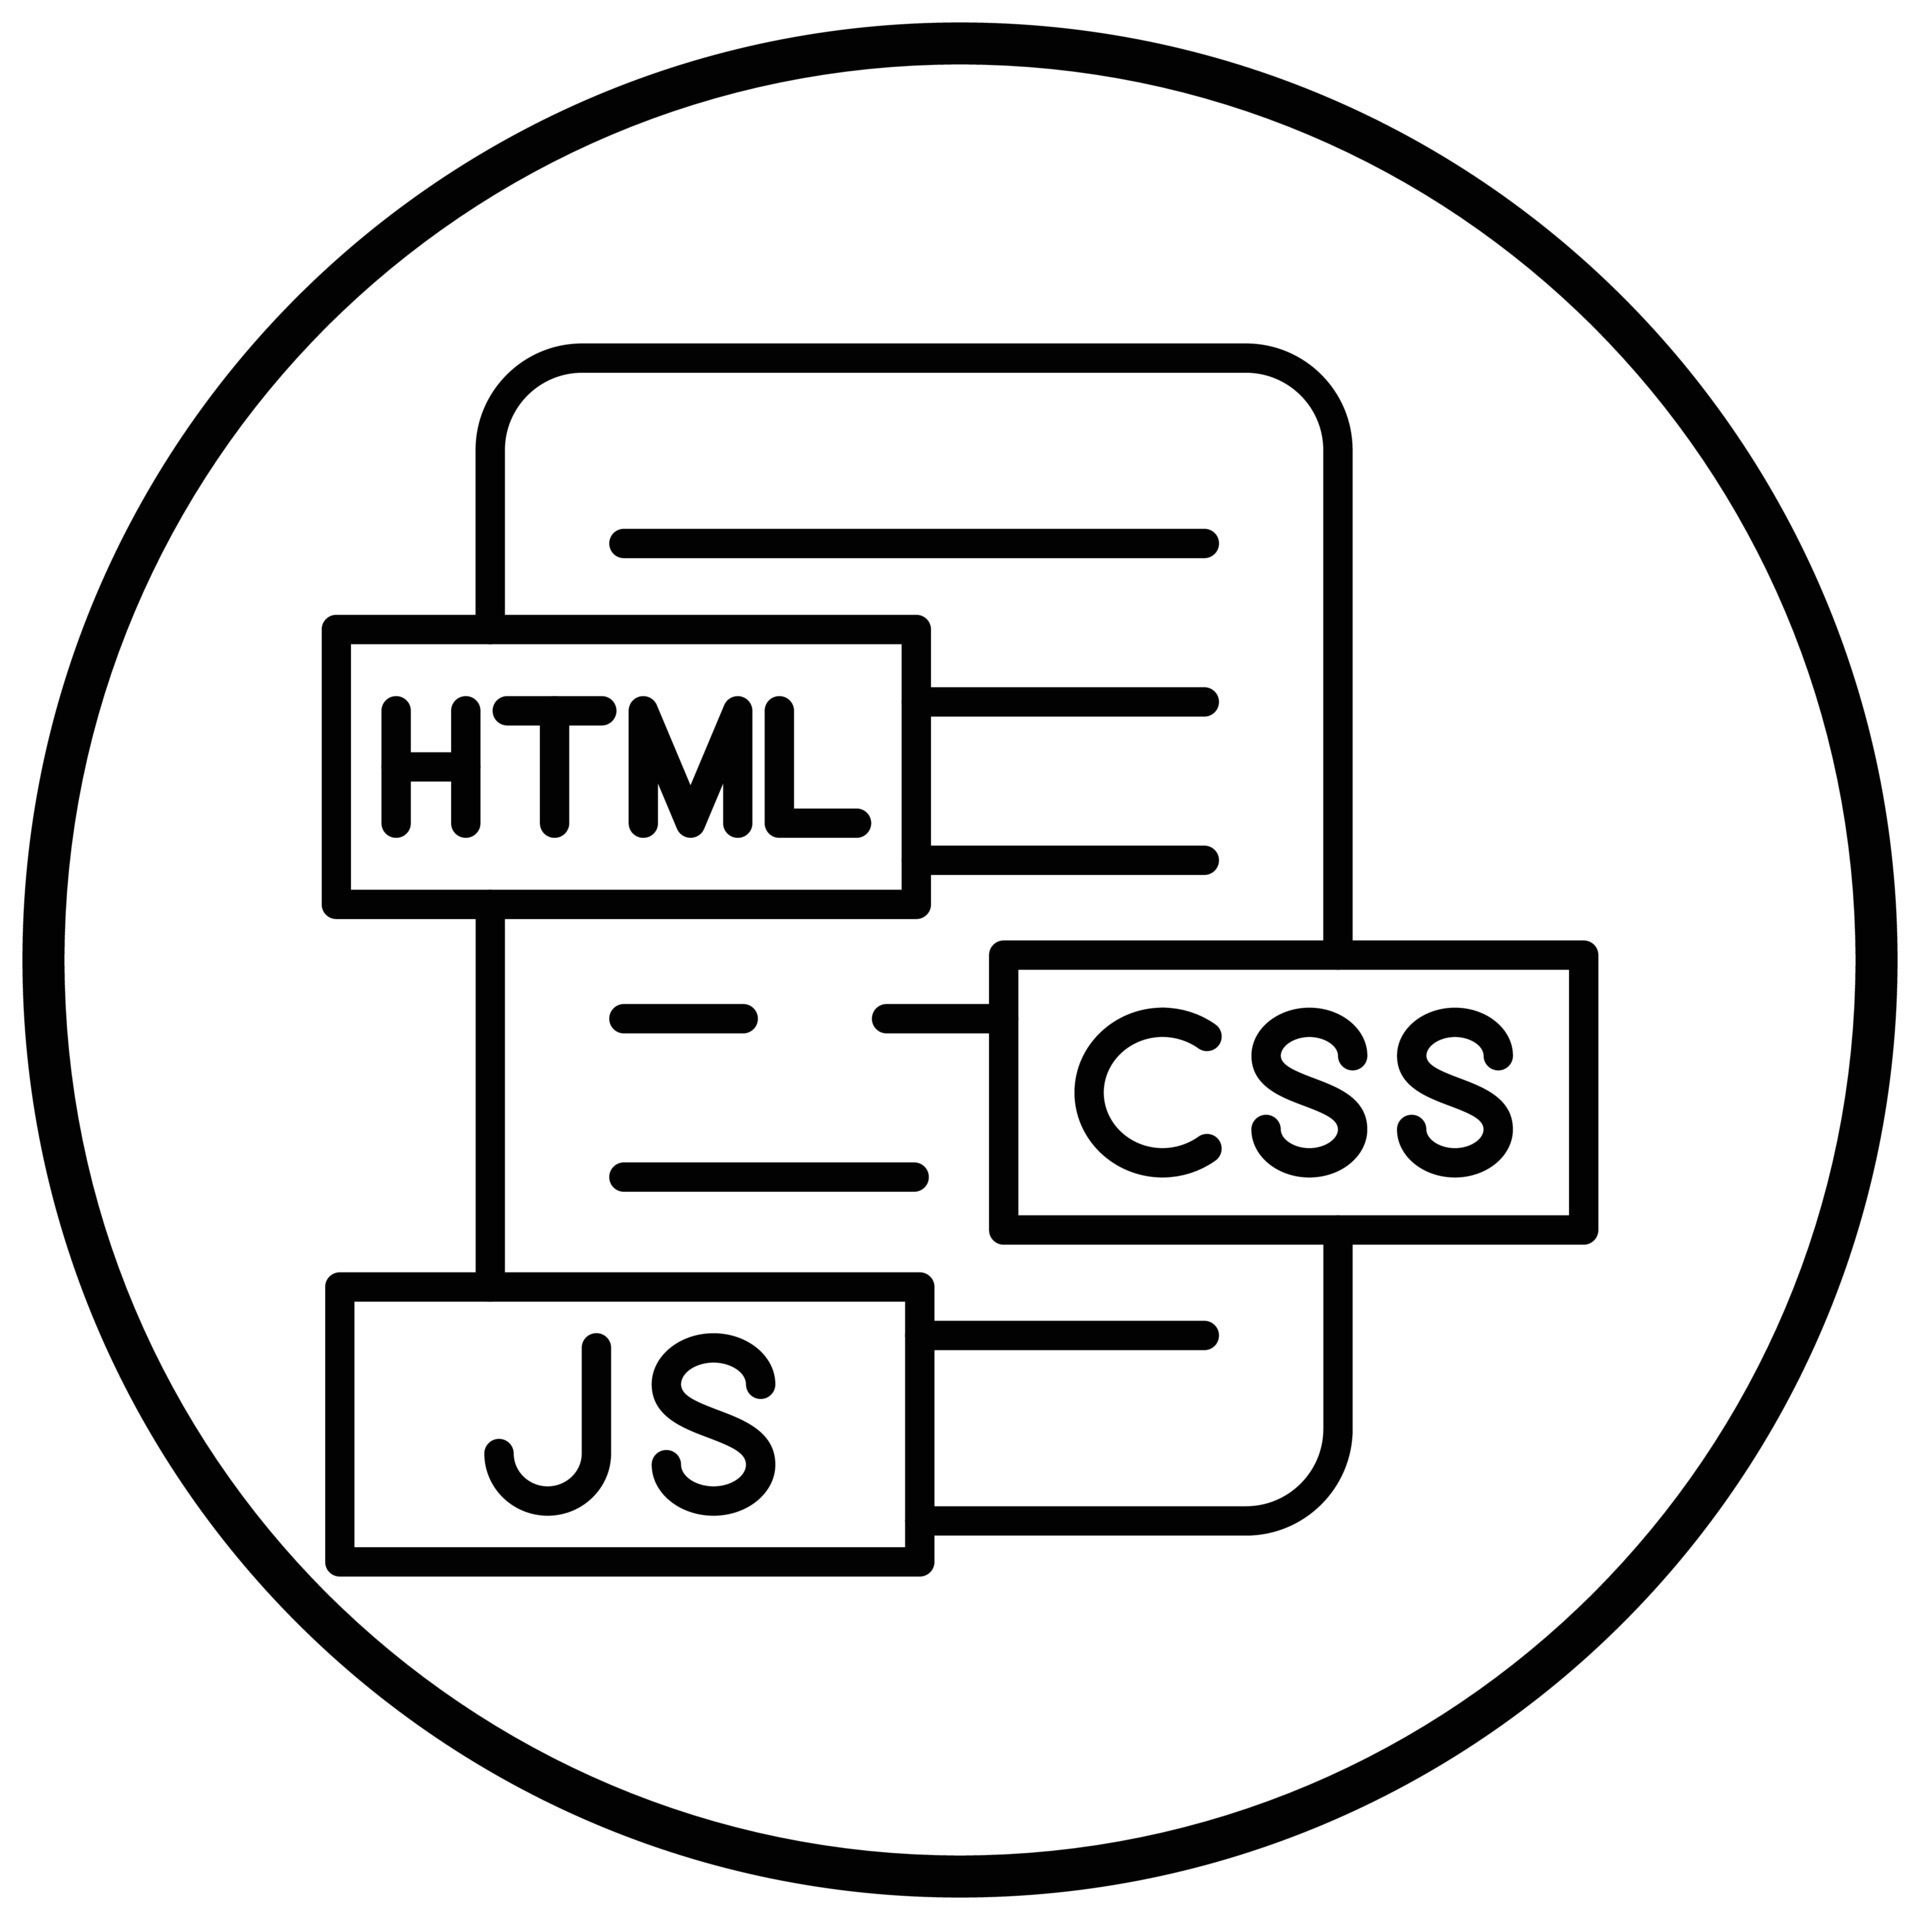
\includegraphics[width=0.5\textwidth]{congnghe.jpg}
    \caption{Công nghệ thiết kết website}
    \label{fig:des_structure}
\end{figure}
  \item \textbf{Thuật toán:} Kiểm tra chuỗi DFA/NFA/NFA$\epsilon$, chuyển đổi NFA $\rightarrow$ DFA, NFA$\epsilon$ $\rightarrow$ NFA, NFA$\epsilon$ $\rightarrow$ DFA, epsilon-closure, xây dựng tập con.
\end{itemize}

\section{Ý nghĩa thực tiễn}
\hspace*{0.7cm}Hệ thống giúp sinh viên củng cố kiến thức về ôtômát, áp dụng công nghệ web vào giảng dạy lý thuyết Tin học, tạo môi trường học tập trực quan, sinh động và dễ tiếp cận. Giảng viên có thể sử dụng để minh họa bài giảng; sinh viên có thể tự học, thực hành và kiểm chứng kết quả mà không cần phần mềm cài đặt phức tạp. Đây là công cụ hữu ích góp phần nâng cao hiệu quả tiếp thu môn học.

\chapter{CƠ SỞ LÝ THUYẾT}
\section{Thuật toán xây dựng tập con (subset construction)}

Cho \(N = (Q_N, \Sigma, \delta_N, q_{0,N}, F_N)\) là một NFA có thể có các \(\varepsilon\)-transition.  
Ta xây dựng một DFA \(D = (Q_D, \Sigma, \delta_D, q_{0,D}, F_D)\) sao cho \(L(D) = L(N)\).

\paragraph{Ý tưởng}  
Mỗi trạng thái của \(D\) là một tập con \(S \subseteq Q_N\) — biểu diễn tập các trạng thái NFA mà N có thể đang ở sau khi đọc một tiền tố của chuỗi đầu vào. Nếu NFA có \(\varepsilon\)-transition, trước và sau mỗi bước đọc ký tự ta phải lấy \emph{\(\varepsilon\)-closure} của các trạng thái.

\paragraph{Định nghĩa phụ}  
Với \(T \subseteq Q_N\), định nghĩa \(\varepsilon\)-closure:
\[
\mathsf{EpsClose}(T) = \{\, q \in Q_N \mid \exists p \in T \text{ sao cho } p \xRightarrow{\varepsilon} q \,\},
\]
tức là tập tất cả trạng thái có thể đạt được từ \(T\) bằng một dãy gồm các \(\varepsilon\)-transition (bao gồm cả \(T\) chính nó).

\paragraph{Cấu thành DFA}
\begin{itemize}
  \item \(Q_D \subseteq \mathcal{P}(Q_N)\) (các trạng thái khả dĩ là các tập con của \(Q_N\)). Thực tế ta chỉ xây những tập con xuất hiện trong quá trình khám phá từ trạng thái khởi đầu.
  \item Trạng thái bắt đầu:
  \[
  q_{0,D} = \mathsf{EpsClose}(\{q_{0,N}\}).
  \]
  \item Hàm chuyển:
  \[
  \delta_D(S, a) = \mathsf{EpsClose}\Big( \bigcup_{q \in S} \delta_N(q,a) \Big),
  \qquad S \subseteq Q_N,\ a\in\Sigma.
  \]
  (Ở đây \(\delta_N(q,a)\) là tập trạng thái NFA đến được từ \(q\) khi đọc ký tự \(a\).)
  \item Tập trạng thái chấp nhận:
  \[
  F_D = \{\, S \subseteq Q_N \mid S \cap F_N \neq \varnothing \,\}.
  \]
  (Một trạng thái tập con là chấp nhận nếu chứa ít nhất một trạng thái chấp nhận của NFA.)
\end{itemize}

\paragraph{Chú ý cài đặt}
\begin{itemize}
  \item Người thực hiện thường biểu diễn các tập con \(S\) bằng bitset hoặc cấu trúc hashable để kiểm tra đã thăm hay chưa.
  \item Nếu NFA không có \(\varepsilon\)-transition, bỏ qua bước \(\mathsf{EpsClose}\).
  \item Số trạng thái \(Q_D\) lý thuyết có thể lên tới \(2^{|Q_N|}\), nhưng thực tế chỉ những tập xuất hiện mới được tạo.
\end{itemize}

\paragraph{Bằng chứng đúng đắn (sketch)}  
Định nghĩa \( \hat{\delta}_N(q, x) \) là tập trạng thái mà NFA có thể đạt được khi bắt đầu ở \(q\) và đọc chuỗi \(x\) (có xét cả \(\varepsilon\)-transition). Mở rộng cho tập \(S\subseteq Q_N\):
\[
\hat{\delta}_N(S,x) = \bigcup_{q\in S} \hat{\delta}_N(q,x).
\]
Ta chứng minh bằng quy nạp theo chiều dài \(x\) rằng trạng thái DFA thu được từ \(q_{0,D}\) bằng cách áp dụng \(\delta_D\) với chuỗi \(x\) là đúng \(\mathsf{EpsClose}(\hat{\delta}_N(\{q_{0,N}\}, x))\).  
Từ đó:
\[
x \in L(N) \iff \hat{\delta}_N(\{q_{0,N}\},x) \cap F_N \neq \varnothing
\]
\[
\iff \mathsf{EpsClose}(\hat{\delta}_N(\{q_{0,N}\},x)) \cap F_N \neq \varnothing
\]
\[
\iff \text{trạng thái DFA sau đọc } x \in F_D
\]
nên \(L(D)=L(N)\).

\paragraph{Phân tích độ phức tạp}
\begin{itemize}
  \item Trong tồi tệ nhất, số trạng thái của DFA là \(O(2^{|Q_N|})\). Mỗi trạng thái có |Σ| cung cấp tối đa |Q_N| thao tác hợp tập (trong cài đặt bitset mỗi bước là \(O(|Q_N|/w)\) với w kích thước machine word).
  \item Thời gian tổng cộng trong tệ nhất \(O(|\Sigma|\cdot |Q_N|\cdot 2^{|Q_N|})\). Tuy nhiên trên thực tế nhiều tập con không xuất hiện nên thường chạy nhanh hơn.
\end{itemize}

\paragraph{Ví dụ nhanh}  
Với NFA đơn giản: \(Q_N=\{q_0,q_1\}\), \(\Sigma=\{a\}\), chuyển: \(q_0 \xrightarrow{a} q_0,q_1\), bắt đầu \(q_0\), chấp nhận \(F_N=\{q_1\}\). Ta có:
\[
q_{0,D}=\{q_0\},\quad
\delta_D(\{q_0\},a)=\{q_0,q_1\},\quad
\delta_D(\{q_0,q_1\},a)=\{q_0,q_1\}.
\]
Do đó DFA có hai trạng thái \(\{\ q_0\ \}\) và \(\{\ q_0,q_1\ \}\), trạng thái chấp nhận là \(\{\ q_0,q_1\ \}\).

\bigskip

\section{Định nghĩa và ký hiệu cơ bản về Automata hữu hạn}
\subsection{Deterministic Finite Automaton (DFA)}

\textbf{Định nghĩa:}  
Một \textbf{DFA} là một ôtômát hữu hạn xác định, được định nghĩa bởi 5 thành phần:
\[
DFA = (Q, \Sigma, \delta, q_0, F)
\]
trong đó:
\begin{itemize}
    \item $Q$ là tập hữu hạn các trạng thái.
    \item $\Sigma$ là tập ký hiệu đầu vào (alphabet).
    \item $\delta: Q \times \Sigma \rightarrow Q$ là hàm chuyển trạng thái xác định.
    \item $q_0 \in Q$ là trạng thái bắt đầu.
    \item $F \subseteq Q$ là tập các trạng thái kết thúc (accepting states).
\end{itemize}

\textbf{Nguyên tắc hoạt động:}  
\begin{itemize}
    \item Với mỗi ký hiệu đầu vào $a \in \Sigma$, từ trạng thái $q$ sẽ chuyển sang đúng một trạng thái tiếp theo $\delta(q,a)$.
    \item Chuỗi $w = a_1 a_2 \dots a_n \in \Sigma^*$ được chấp nhận nếu hàm mở rộng $\hat{\delta}(q_0, w) \in F$.
\end{itemize}

\textbf{Hàm chuyển mở rộng:}  
\[
\hat{\delta}: Q \times \Sigma^* \rightarrow Q
\]
được định nghĩa đệ quy:
\[
\hat{\delta}(q, \epsilon) = q
\]
\[
\hat{\delta}(q, xa) = \delta(\hat{\delta}(q, x), a), \quad x \in \Sigma^*, a \in \Sigma
\]

\textbf{Ngôn ngữ được chấp nhận:}  
Ngôn ngữ của DFA $M$ được định nghĩa là tập tất cả các chuỗi mà DFA chấp nhận:
\[
L(M) = \{ w \in \Sigma^* \mid \hat{\delta}(q_0, w) \in F \}.
\]

\textbf{Tính chất quan trọng của DFA:}
\begin{itemize}
    \item Với mỗi trạng thái và ký tự đầu vào, có \textbf{chính xác một} trạng thái tiếp theo.
    \item Ngôn ngữ chấp nhận bởi DFA luôn là \textbf{ngôn ngữ chính quy (regular language)}.
    \item DFA có thể được tối tiểu hóa thành DFA tối tiểu duy nhất (đến đẳng cấu) bằng thuật toán Hopcroft.
    \item Ngôn ngữ chính quy đóng với các phép toán: hợp, giao, bù, hiệu, nối (concatenation), lặp Kleene ($*$).
\end{itemize}

\textbf{Ví dụ minh họa:} Xét ngôn ngữ trên bảng chữ cái $\{a, b\}$ gồm các chuỗi mà
chữ $a$ :  $L=(ab)^{*}aa b^{*}$:
\[
aa,\qquad abaa,\qquad ababaa bbb.
\]



\begin{center}
\begin{tikzpicture}[->,>=stealth,shorten >=1pt,auto,node distance=2.5cm,semithick]
  \tikzstyle{every state}=[fill=blue!20,draw=black,text=black]

  \node[state,initial] (q0) {$q_0$};
  \node[state] (q1) [right of=q0] {$q_1$};
  \node[state,accepting] (q2) [right of=q1] {$q_2$};

  \path (q0) edge [bend left] node {a} (q1)
        (q1) edge [bend left] node {b} (q0)
        (q1) edge node {a} (q2)
        (q2) edge [loop above] node {b} ();
\end{tikzpicture}
\end{center}

\textbf{Chạy DFA:}  
Ví dụ với chuỗi $w = aab$:
\[
\hat{\delta}(q_0, a) = q_1, \quad \hat{\delta}(q_1, a) = q_2, \quad \hat{\delta}(q_2, b) = q_2 \in F
\]
→ Chuỗi được chấp nhận.

\textbf{Thuật toán kiểm tra chuỗi:}  
\begin{enumerate}
    \item Khởi tạo trạng thái hiện tại $q = q_0$.
    \item Duyệt từng ký tự $a_i$ trong chuỗi $w$:
    \[
        q \leftarrow \delta(q, a_i)
    \]
    \item Nếu $q \in F$ sau khi hết chuỗi → chuỗi được chấp nhận.
\end{enumerate}

\textbf{Tối tiểu hóa DFA:}  
- Loại bỏ các trạng thái không thể tới được (unreachable).
- Gom các trạng thái tương đương (cùng dẫn tới chấp nhận/không chấp nhận giống nhau).
- Thuật toán Hopcroft: phân hoạch trạng thái thành các lớp tương đương, tạo DFA tối tiểu.
Bên trái là DFA ban đầu, có thể có các trạng thái không cần thiết hoặc tương đương.  
Bên phải là DFA tối tiểu sau khi loại bỏ trạng thái không thể tới và gom các trạng thái tương đương (Hopcroft).

\subsection{Non-Deterministic Finite Automaton (NFA)}

\textbf{Định nghĩa:}  
Một \textbf{NFA} là ôtômát hữu hạn không xác định, được định nghĩa bởi 5 thành phần:
\[
NFA = (Q, \Sigma, \delta, q_0, F)
\]
trong đó:
\begin{itemize}
    \item $Q$ là tập hữu hạn các trạng thái.
    \item $\Sigma$ là tập ký hiệu đầu vào (alphabet).
    \item $\delta: Q \times \Sigma \rightarrow P(Q)$ là hàm chuyển trạng thái, mỗi cặp $(q, a)$ có thể dẫn tới nhiều trạng thái.
    \item $q_0 \in Q$ là trạng thái bắt đầu.
    \item $F \subseteq Q$ là tập các trạng thái kết thúc (accepting states).
\end{itemize}

\textbf{Nguyên tắc hoạt động:}  
\begin{itemize}
    \item Tại một trạng thái $q$ và ký tự đầu vào $a \in \Sigma$, NFA có thể chuyển sang \textbf{một hoặc nhiều trạng thái} trong $\delta(q,a)$.
    \item Chuỗi $w = a_1 a_2 \dots a_n$ được chấp nhận nếu tồn tại ít nhất một chuỗi trạng thái:
    \[
        q_0 \xrightarrow{a_1} q_1 \xrightarrow{a_2} \dots \xrightarrow{a_n} q_n \in F
    \]
\end{itemize}

\textbf{Hàm mở rộng:}  
Hàm mở rộng $\hat{\delta}: Q \times \Sigma^* \rightarrow P(Q)$ được định nghĩa bằng:
\[
\hat{\delta}(q, \epsilon) = \{q\}
\]
\[
\hat{\delta}(q, xa) = \bigcup_{p \in \hat{\delta}(q, x)} \delta(p, a), \quad x \in \Sigma^*, a \in \Sigma
\]
\textbf{Ví dụ:}
Xét NFA gồm ba trạng thái: 
$q_0$ là trạng thái bắt đầu, $q_1$ là trạng thái trung gian, 
và $q_2$ là trạng thái chấp nhận. 

Tại trạng thái $q_0$, ký tự $b$ được phép xuất hiện nhiều lần 
(vòng lặp trên chính nó), trong khi ký tự $a$ sẽ đưa NFA sang 
trạng thái $q_1$. Từ $q_1$, ký tự $b$ sẽ chuyển NFA sang trạng thái 
chấp nhận $q_2$. Khi đã vào $q_2$, tự động cho phép đọc tuỳ ý 
các ký tự $a$ hoặc $b$ (vòng lặp trên cả hai ký tự).
\\
Muốn vào trạng thái chấp nhận $q_2$, ta phải đi qua các bước:

\begin{itemize}
    \item Bất kỳ số lượng ký tự $b$ ở trạng thái $q_0$:
    \[
        b^{*}
    \]
    \item Một ký tự $a$ để chuyển sang trạng thái $q_1$:
    \[
        a
    \]
    \item Một ký tự $b$ để chuyển sang trạng thái $q_2$:
    \[
        b
    \]
    \item Sau khi vào trạng thái $q_2$, được phép đọc tùy ý các ký tự $a$ hoặc $b$:
    \[
        (a + b)^{*}
    \]
\end{itemize}

Do đó, ngôn ngữ mà NFA này chấp nhận là:
\[
L = b^{*}\, a\, b\, (a+b)^{*}.
\]


\begin{center}
\begin{tikzpicture}[->,>=stealth,shorten >=1pt,auto,node distance=2.5cm,semithick]
  \tikzstyle{every state}=[fill=orange!20,draw=black,text=black]

  \node[state,initial] (q0) {$q_0$};
  \node[state] (q1) [right of=q0] {$q_1$};
  \node[state,accepting] (q2) [right of=q1] {$q_2$};

  % Chuyển trạng thái
  \path (q0) edge [bend left] node {a} (q1)
        (q0) edge [loop above] node {b} ()
        (q1) edge node {a} (q2)
        (q1) edge node {b} (q2)
        (q2) edge [loop above] node {a,b} ();
\end{tikzpicture}
\end{center}

\textbf{Ghi chú:}
\begin{itemize}
    \item Mỗi ký tự đầu vào có thể dẫn tới nhiều trạng thái.  
    \item NFA có thể chấp nhận một chuỗi nếu tồn tại ít nhất một đường đi từ trạng thái bắt đầu đến trạng thái kết thúc.  
    \item NFA luôn có thể được chuyển đổi sang DFA bằng thuật toán \textbf{subset construction}.
\end{itemize}

\subsection{Non-Deterministic Finite Automaton với epsilon (NFA$\epsilon$)}
\textbf{Định nghĩa:}  
Một \textbf{NFA$\epsilon$} là ôtômát hữu hạn không xác định, cho phép chuyển trạng thái mà không cần đọc ký hiệu đầu vào (chuyển $\epsilon$), được định nghĩa bởi 5 thành phần:
\[
NFA\epsilon = (Q, \Sigma, \delta, q_0, F)
\]
trong đó:
\begin{itemize}
    \item $Q$ là tập hữu hạn các trạng thái.
    \item $\Sigma$ là tập ký hiệu đầu vào (alphabet).
    \item $\delta: Q \times (\Sigma \cup \{\epsilon\}) \rightarrow P(Q)$ là hàm chuyển trạng thái, mỗi cặp $(q,a)$ hoặc $(q,\epsilon)$ có thể dẫn tới nhiều trạng thái.
    \item $q_0 \in Q$ là trạng thái bắt đầu.
    \item $F \subseteq Q$ là tập các trạng thái kết thúc (accepting states).
\end{itemize}

\textbf{Nguyên tắc hoạt động:}  
\begin{itemize}
    \item Tại một trạng thái $q$, NFA$\epsilon$ có thể:
    \begin{itemize}
        \item Chuyển sang các trạng thái trong $\delta(q, a)$ nếu đọc ký hiệu $a \in \Sigma$.
        \item Chuyển sang các trạng thái trong $\delta(q, \epsilon)$ mà không tiêu thụ ký hiệu đầu vào (epsilon-transition).
    \end{itemize}
    \item Một chuỗi $w \in \Sigma^*$ được chấp nhận nếu tồn tại ít nhất một đường đi từ $q_0$ đến trạng thái $q_f \in F$ theo các ký hiệu trong $w$ và có thể xen kẽ các chuyển $\epsilon$.
\end{itemize}

\textbf{Hàm mở rộng:}  
Hàm mở rộng $\hat{\delta}: Q \times \Sigma^* \rightarrow P(Q)$ được định nghĩa bằng:
\[
\hat{\delta}(q, \epsilon) = \epsilon\text{-closure}(q)
\]
\[
\hat{\delta}(q, xa) = \bigcup_{p \in \hat{\delta}(q, x)} \epsilon\text{-closure}(\delta(p, a)), \quad x \in \Sigma^*, a \in \Sigma
\]

Trong đó, \textbf{$\epsilon$-closure} của một trạng thái $q$, ký hiệu $\epsilon\text{-closure}(q)$, là tập tất cả các trạng thái có thể đạt được từ $q$ chỉ bằng các chuyển $\epsilon$ (bao gồm chính $q$).

\textbf{Ví dụ trực quan:}  

\begin{center}
\begin{tikzpicture}[->,>=stealth,shorten >=1pt,auto,node distance=2.5cm,semithick]
  \tikzstyle{every state}=[fill=orange!20,draw=black,text=black]

  \node[state,initial] (q0) {$q_0$};
  \node[state] (q1) [right of=q0] {$q_1$};
  \node[state,accepting] (q2) [right of=q1] {$q_2$};
  \node[state] (q3) [below of=q1] {$q_3$};

  % Chuyển trạng thái
  \path (q0) edge node {a} (q1)
        (q1) edge node {b} (q2)
        (q1) edge [bend left] node {$\epsilon$} (q3)
        (q3) edge node {a} (q2)
        (q2) edge [loop right] node {b} ();
\end{tikzpicture}
\end{center}

\textbf{Ghi chú:}  
\begin{itemize}
    \item Trạng thái $q_1$ có thể đi tới $q_3$ mà không cần đọc ký hiệu ($\epsilon$-transition).  
    \item Chuỗi $aa b$ có thể được chấp nhận nhờ việc di chuyển qua $\epsilon$ từ $q_1$ sang $q_3$.  
    \item NFA$\epsilon$ có thể được chuyển đổi sang DFA (không epsilon) bằng thuật toán epsilon-closure và subset construction.
\end{itemize}
\section{Chuyển đổi NFA sang DFA}
\begin{center}
\begin{tikzpicture}[->,>=stealth,shorten >=1pt,auto,node distance=3cm,semithick]
  \tikzstyle{every state}=[fill=red!20,draw=black,text=black]

  \node[state,initial] (S0) {$\{p_0\}$};
  \node[state] (S1) [right of=S0] {$\{p_1,p_2\}$};
  \node[state,accepting] (S2) [below of=S0] {$\{p_2\}$};

  \path (S0) edge node {a} (S1)
        (S1) edge node {b} (S2)
        (S2) edge [loop below] node {a,b} ();
\end{tikzpicture}
\end{center}

\section{Chuyển NFA$\epsilon$ sang NFA hoặc DFA}

\begin{center}
\begin{tikzpicture}[->,>=Stealth,shorten >=1pt,auto,node distance=2.5cm,semithick]

\tikzstyle{nfae}=[state,fill=yellow!20,minimum width=1.5cm,minimum height=1cm]
\tikzstyle{nfa}=[state,fill=green!20,minimum width=1.5cm,minimum height=1cm]
\tikzstyle{dfa}=[state,fill=red!20,minimum width=2cm,minimum height=1cm]

% ===== NFAε (hàng trên) =====
\node[nfae,initial] (r0) {$r_0$};
\node[nfae] (r1) [right=of r0] {$r_1$};
\node[nfae,accepting] (r2) [right=of r1] {$r_2$};

\path (r0) edge node[above] {a} (r1)
      (r0) edge [bend left] node[above] {$\epsilon$} (r2)
      (r1) edge node[above] {b} (r2)
      (r2) edge [loop above] node {a,b} ();

% ===== NFA (hàng giữa) =====
\node[nfa] (n0) [below=3cm of r0] {$q_0$};
\node[nfa] (n1) [below=3cm of r1] {$q_1$};
\node[nfa,accepting] (n2) [below=3cm of r2] {$q_2$};

\path (n0) edge node[below] {a} (n1)
      (n0) edge [bend left] node[below] {b} (n2)
      (n1) edge node[below] {b} (n2)
      (n2) edge [loop below] node {a,b} ();

% Mũi tên nối NFAε → NFA
\draw[->,dashed] (r0) -- (n0) node[midway,left] {ε-closure};
\draw[->,dashed] (r1) -- (n1) node[midway,left] {ε-closure};
\draw[->,dashed] (r2) -- (n2) node[midway,left] {ε-closure};

% ===== DFA (hàng dưới cùng) =====
\node[dfa] (S0) [below=3cm of n0] {$\{r_0,r_2\}$};
\node[dfa] (S1) [below=3cm of n1] {$\{r_1,r_2\}$};
\node[dfa,accepting] (S2) [below=3cm of n2] {$\{r_2\}$};

\path (S0) edge node[below] {a} (S1)
      (S0) edge [bend left] node[below] {b} (S2)
      (S1) edge node[below] {b} (S2)
      (S1) edge [bend left] node[below] {a} (S2)
      (S2) edge [loop below] node {a,b} ();

% Mũi tên nối NFAε → DFA
\draw[->, dotted] (r0) -- (S0) node[midway,left] {Subset};
\draw[->, dotted] (r1) -- (S1) node[midway,left] {Subset};
\draw[->, dotted] (r2) -- (S2) node[midway,left] {Subset};

\end{tikzpicture}
\end{center}
\subsection{Epsilon-closure (E-closure)}

\textbf{Định nghĩa:}  
Epsilon-closure của một trạng thái $q$ trong NFA$\epsilon$, ký hiệu $E(q)$, là tập tất cả các trạng thái mà NFA$\epsilon$ có thể tới từ $q$ bằng \textbf{một hoặc nhiều phép chuyển $\epsilon$}, bao gồm chính $q$:
\[
E(q) = \{ p \in Q \mid q \xrightarrow{\epsilon*} p \}
\]

\textbf{Ví dụ:} nếu $q_0 \xrightarrow{\epsilon} q_1 \xrightarrow{\epsilon} q_2$, thì $E(q_0) = \{q_0, q_1, q_2\}$.  

\textbf{Ý nghĩa:}  
- Epsilon-closure giúp loại bỏ các chuyển epsilon khi chuyển NFA$\epsilon$ sang NFA thông thường.  
- Sau khi loại bỏ epsilon, NFA chỉ còn các chuyển trạng thái theo ký hiệu trong $\Sigma$.

\subsection{Thuật toán chuyển NFA$\epsilon$ sang NFA}

\begin{enumerate}
    \item \textbf{Tính epsilon-closure cho mỗi trạng thái:}  
    \[
        \forall q \in Q, \quad E(q) = \text{tập tất cả các trạng thái có thể tới từ $q$ bằng epsilon}
    \]
    
    \item \textbf{Xây dựng hàm chuyển mới $\delta'$:}  
    Với mỗi ký tự $a \in \Sigma$ và trạng thái $q \in Q$, tập trạng thái kế tiếp được xác định bằng:
    \[
        \delta'(q, a) = \bigcup_{p \in E(q)} \delta(p, a)
    \]
    - Ở đây, $\delta(p,a)$ là các trạng thái NFAε có thể tới từ $p$ với ký tự $a$.
    - $\delta'$ loại bỏ epsilon, chỉ còn chuyển theo ký tự trong $\Sigma$.
    
    \item \textbf{Xác định trạng thái kết thúc:}  
    Một trạng thái $q$ trong NFA mới là trạng thái kết thúc nếu epsilon-closure của nó chứa ít nhất một trạng thái kết thúc trong NFA$\epsilon$:
    \[
        q \in F' \iff E(q) \cap F \neq \emptyset
    \]
\end{enumerate}

\subsection{Thuật toán chuyển NFA$\epsilon$ sang DFA}

Quy trình tổng quát gồm 2 bước chính:

\begin{enumerate}
    \item \textbf{Bước 1: Chuyển NFA$\epsilon$ sang NFA}  
    - Dùng epsilon-closure để loại bỏ các chuyển epsilon như hướng dẫn ở trên.  
    - Kết quả là NFA thông thường chỉ có các chuyển theo ký hiệu trong $\Sigma$.
    
    \item \textbf{Bước 2: Chuyển NFA sang DFA (Subset Construction)}  
    \begin{enumerate}
        \item Mỗi trạng thái DFA là một tập con các trạng thái NFA.
        \item Trạng thái bắt đầu DFA: $\{ q_0 \}$ hoặc epsilon-closure của $q_0$ nếu xuất phát từ NFA$\epsilon$.  
        \item Hàm chuyển DFA: với tập con $S \subseteq Q$ và ký tự $a \in \Sigma$, tập trạng thái kế tiếp là:
        \[
            \delta_D(S, a) = \bigcup_{q \in S} \delta'(q, a)
        \]
        \item Trạng thái kết thúc DFA: mọi tập con chứa ít nhất một trạng thái kết thúc của NFA.
    \end{enumerate}
\end{enumerate}

\textbf{Lưu ý:}
\begin{itemize}
    \item Subset construction có thể tạo ra tối đa $2^{|Q|}$ trạng thái DFA, nhưng thường ít hơn nhiều vì nhiều tập con không bao giờ xuất hiện.  
    \item Kết quả là một DFA chấp nhận cùng ngôn ngữ với NFA$\epsilon$ ban đầu.
\end{itemize}


\section{Kiểm tra chuỗi trong DFA, NFA, NFA$\epsilon$}

\begin{center}
\begin{tikzpicture}[
    node distance=0.4cm,
    every node/.style={rectangle, draw, rounded corners, align=center, text width=4.5cm, minimum height=0.8cm},
    >=stealth
]

% DFA
\node[fill=blue!20] (dfa0) {DFA};
\node[below=0.3cm of dfa0] (dfa1) {Đọc ký hiệu tuần tự $a_1 a_2 ... a_n$};
\node[below=0.3cm of dfa1] (dfa2) {Duy nhất một đường đi};
\node[below=0.3cm of dfa2] (dfa3) {Chấp nhận nếu trạng thái cuối cùng $\in F$};

% NFA
\node[fill=orange!20, right=1cm of dfa0] (nfa0) {NFA};
\node[below=0.3cm of nfa0] (nfa1) {Mỗi ký hiệu có nhiều trạng thái khả thi};
\node[below=0.3cm of nfa1] (nfa2) {Duyệt tất cả đường đi khả thi};
\node[below=0.3cm of nfa2] (nfa3) {Chấp nhận nếu ít nhất một đường tới $F$};

% NFA epsilon
\node[fill=green!20, right=1cm of nfa0] (nfae0) {NFA$\epsilon$};
\node[below=0.3cm of nfae0] (nfae1) {Mở rộng $\epsilon$-closure trước khi đọc ký hiệu};
\node[below=0.3cm of nfae1] (nfae2) {Sau đó kiểm tra như NFA};
\node[below=0.3cm of nfae2] (nfae3) {Chấp nhận nếu tồn tại đường tới $F$};

% Mũi tên dọc trong từng cột
\foreach \x/\y in {dfa1/dfa2, dfa2/dfa3, nfa1/nfa2, nfa2/nfa3, nfae1/nfae2, nfae2/nfae3} {
    \draw[->] (\x.south) -- (\y.north);
}

\end{tikzpicture}
\end{center}


\text{Ví dụ kiểm tra chuỗi $w = ab$ trên DFA, NFA, NFA$\epsilon$}

\begin{center}
\begin{tikzpicture}[->,>=stealth,shorten >=1pt,auto,node distance=2cm,semithick]

% ---------------- DFA ----------------
\node[rectangle, draw, fill=blue!20] (dfa0) {DFA: $q_0$ (bắt đầu)};
\node[rectangle, draw, fill=blue!10, right=2cm of dfa0] (dfa1) {$q_1$ (sau 'a')};
\node[rectangle, draw, fill=green!20, right=2cm of dfa1] (dfa2) {$q_2$ (sau 'ab', kết thúc)};

% Mũi tên DFA
\draw[->] (dfa0) -- node[above]{a} (dfa1);
\draw[->] (dfa1) -- node[above]{b} (dfa2);

% ---------------- NFA ----------------
\node[rectangle, draw, fill=orange!20, below=3cm of dfa0] (nfa0) {NFA: $p_0$ (bắt đầu)};
\node[rectangle, draw, fill=orange!10, right=2cm of nfa0] (nfa1a) {$p_1$ (sau 'a')};
\node[rectangle, draw, fill=orange!10, below=0.8cm of nfa1a] (nfa1b) {$p_2$ (sau 'a')};
\node[rectangle, draw, fill=green!20, right=2cm of nfa1a] (nfa2a) {$p_3$ (sau 'ab', kết thúc)};
\node[rectangle, draw, fill=green!20, right=2cm of nfa1b] (nfa2b) {$p_3$ (sau 'ab', kết thúc)};

% Mũi tên NFA
\draw[->] (nfa0) -- node[above]{a} (nfa1a);
\draw[->] (nfa0.east) -- ++(0.2,0) -- ++(0,-0.8) -- (nfa1b.west) node[midway,left]{a};
\draw[->] (nfa1a) -- node[above]{b} (nfa2a);
\draw[->] (nfa1b) -- node[below]{b} (nfa2b);

% ---------------- NFA epsilon ----------------
\node[rectangle, draw, fill=cyan!20, below=3cm of nfa0] (nfae0) {NFA$\epsilon$: $r_0$ (bắt đầu)};
\node[rectangle, draw, fill=cyan!10, right=2cm of nfae0] (nfae1) {$r_1$ (sau epsilon + 'a')};
\node[rectangle, draw, fill=green!20, right=2cm of nfae1] (nfae2) {$r_2$ (sau 'b', kết thúc)};

% Mũi tên NFA epsilon
\draw[->] (nfae0) -- node[above]{\(\epsilon\)} (nfae1);
\draw[->] (nfae1) -- node[above]{b} (nfae2);

\end{tikzpicture}
\end{center}

\newpage
\chapter{THIẾT KẾ VÀ CÀI ĐẶT HỆ THỐNG}

\section{Thiết kế hệ thống}
\hspace*{0.7cm}Hệ thống được thiết kế theo mô hình \textbf{client-server} với frontend đảm nhiệm giao diện người dùng và backend xử lý thuật toán ôtômát. Kiến trúc hệ thống bao gồm:
\begin{itemize}
  \item \textbf{Frontend:} hiển thị đồ thị ôtômát, cung cấp giao diện nhập dữ liệu và kiểm tra chuỗi, sử dụng \texttt{vis\_network.js} để trực quan hóa.
  \item \textbf{Backend:} xử lý thuật toán kiểm tra chuỗi, chuyển đổi NFA/NFA$\epsilon$ sang DFA, tính epsilon-closure, xây dựng tập con.
  \item \textbf{Lưu trữ dữ liệu:} LocalStorage dùng để lưu trữ ôtômát người dùng đã nhập, cho phép tải lại khi cần.
\end{itemize}

\section{Thiết kế giao diện}
\begin{itemize}
  \item \textbf{Trang nhập ôtômát:} form nhập trạng thái, ký hiệu đầu vào, bảng chuyển.
  \item \textbf{Trang kiểm tra chuỗi:} nhập chuỗi đầu vào, hiển thị các bước chuyển trạng thái, tô màu trạng thái đang được xử lý.
  \item \textbf{Trang chuyển đổi ôtômát:} chọn loại chuyển đổi, hiển thị kết quả đồ thị sau chuyển đổi.
  \item \textbf{Trang bài tập luyện tập:} sinh viên có thể thử nghiệm với bài tập ngẫu nhiên và so sánh đáp án.
\end{itemize}

\section{Thiết kế dữ liệu}
\begin{figure}[H]
\centering
\begin{tikzpicture}[
    bubble/.style={
        circle,
        draw,
        minimum size=2.2cm,
        align=center,
        font=\small,
        fill=blue!5
    },
    line/.style={-stealth, thick}
]

% Main bubble
\node[bubble, fill=yellow!20] (auto) {Automaton\\JSON};

% Sub bubbles
\node[bubble, right=3.5cm of auto] (states) {states\\(q0, q1, q2)};
\node[bubble, above right=1.5cm and 3cm of auto] (alphabet) {alphabet\\(a, b)};
\node[bubble, above left=1.5cm and 3cm of auto] (start) {start\\q0};
\node[bubble, left=3.5cm of auto] (accept) {accept\\(q2)};
\node[bubble, below=2cm of auto] (trans) {transitions\\q0→q1…};

% Arrows
\draw[line] (auto) -- (states);
\draw[line] (auto) -- (alphabet);
\draw[line] (auto) -- (start);
\draw[line] (auto) -- (accept);
\draw[line] (auto) -- (trans);

\end{tikzpicture}

\caption{Sơ đồ mô tả dữ liệu ôtômát dạng JSON}
\label{fig:json_bubble}
\end{figure}


\section{Thuật toán chính}

\hspace*{0.7cm}\textbf{1. Kiểm tra chuỗi}
Chức năng cho phép người dùng nhập một chuỗi để xác định xem chuỗi có được chấp nhận bởi ôtômát (DFA hoặc NFA) hay không. Hệ thống hiển thị từng bước chuyển trạng thái và làm nổi bật trạng thái hiện tại trên sơ đồ, giúp người học theo dõi trực quan quá trình duyệt.

\textbf{2. Chuyển đổi NFA → DFA}
Hệ thống sử dụng thuật toán \textit{subset construction} để chuyển một NFA sang DFA tương đương. Mỗi trạng thái của DFA được biểu diễn như một tập các trạng thái NFA. Kết quả được xuất ra dưới dạng JSON và sơ đồ DFA với nhãn dạng \{q0, q1\}.

\textbf{3. Chuyển đổi NFA$\epsilon$ → NFA}
Việc loại bỏ các chuyển $\epsilon$ được thực hiện bằng thuật toán \textit{epsilon-closure}. Với mỗi trạng thái, hệ thống tính tập các trạng thái có thể đạt được thông qua một hoặc nhiều bước $\epsilon$, sau đó thay thế các cạnh $\epsilon$ bằng các cạnh tương ứng. Kết quả là một NFA tương đương không còn chuyển $\epsilon$.

\textbf{4. Chuyển đổi NFA$\epsilon$ → DFA}
Quá trình gồm hai bước: (1) loại bỏ các chuyển $\epsilon$ bằng epsilon-closure để thu được NFA không $\epsilon$; (2) áp dụng \textit{subset construction} để tạo ra DFA tương đương. Hệ thống thực hiện tự động và trả về DFA cuối cùng dưới dạng sơ đồ và JSON.



\section{Cài đặt hệ thống}
\begin{figure}[H]
\centering
\begin{tikzpicture}[
    node distance=1.8cm,
    every node/.style={font=\small},
    box/.style={rectangle, draw, rounded corners, align=center, minimum width=5cm, minimum height=1cm},
    arrow/.style={->, thick}
]

% Nodes
\node[box] (input) {Người dùng nhập/tải ôtômát};
\node[box, below of=input] (choose) {Chọn chức năng:\\Kiểm tra chuỗi hoặc Chuyển đổi mô hình};
\node[box, below of=choose] (backend) {Backend xử lý thuật toán\\(DFA/NFA, chuyển đổi, epsilon-closure)};
\node[box, below of=backend] (output) {Trả kết quả dạng JSON};
\node[box, below of=output] (frontend) {Frontend hiển thị đồ thị và các bước chuyển};

% Arrows
\draw[arrow] (input) -- (choose);
\draw[arrow] (choose) -- (backend);
\draw[arrow] (backend) -- (output);
\draw[arrow] (output) -- (frontend);

\end{tikzpicture}
\caption{Sơ đồ quy trình vận hành hệ thống}
\label{fig:flow_system}
\end{figure}
\hspace*{0.7cm}Hệ thống biểu diễn ôtômát dưới dạng đồ thị trạng thái, trong đó mỗi trạng thái được hiển thị bằng một nút có màu sắc phân biệt: trạng thái bắt đầu được tô xanh lá, các trạng thái kết thúc được tô đỏ, và các trạng thái thông thường được tô xanh dương. Các chuyển trạng thái được vẽ dưới dạng mũi tên hướng, thể hiện trực quan cách ôtômát xử lý chuỗi đầu vào.

\begin{figure}[H]
\centering
\begin{tikzpicture}[
    node distance=2.3cm,
    every state/.style={thick, minimum size=11mm}
]

% States dòng 1
\node[state, fill=green!50] (q0) {$q0$};
\node[state, fill=blue!40, right of=q0] (q1) {$q1$};
\node[state, fill=blue!40, right of=q1] (q2) {$q2$};
\node[state, fill=red!60, right of=q2, accepting] (q3) {$q3$};

% States dòng 2
\node[state, fill=blue!40, below of=q1] (q4) {$q4$};
\node[state, fill=blue!40, right of=q4] (q5) {$q5$};
\node[state, fill=blue!40, right of=q5] (q6) {$q6$};
\node[state, fill=red!60, right of=q6, accepting] (q7) {$q7$};

% --- Transitions dòng trên ---
\draw[->, thick] (q0) -- node[above]{a} (q1);
\draw[->, thick] (q1) -- node[above]{b} (q2);
\draw[->, thick] (q2) -- node[above]{a} (q3);

% Vòng lặp
\draw[->, thick] (q1) edge[loop above] node{a,b} ();
\draw[->, thick] (q2) edge[loop above] node{b} ();
\draw[->, thick] (q0) edge[loop above] node{b} ();

% --- Transitions xuống dòng ---
\draw[->, thick] (q1) -- node[left]{a} (q4);
\draw[->, thick] (q2) -- node[right]{b} (q5);
\draw[->, thick] (q3) -- node[right]{a} (q7);

% Kết nối dòng dưới
\draw[->, thick] (q4) -- node[above]{b} (q5);
\draw[->, thick] (q5) -- node[above]{a} (q6);
\draw[->, thick] (q6) -- node[above]{b} (q7);

% Vòng lặp dòng dưới
\draw[->, thick] (q4) edge[loop below] node{a} ();
\draw[->, thick] (q5) edge[loop below] node{b} ();
\draw[->, thick] (q6) edge[loop below] node{a,b} ();

% Liên kết giữa các tầng
\draw[->, thick, dashed] (q3) -- node[right]{ε} (q6);
\draw[->, thick, dashed] (q4) -- node[left]{ε} (q1);

\end{tikzpicture}
\caption{Ôtômát 8 trạng thái với mã màu: start (xanh lá), normal (xanh dương), accept (đỏ).}
\end{figure}

\section{Các hàm hỗ trợ}
\hspace*{0.7cm}\paragraph{Đọc Automata từ văn bản}
 cho phép đọc một chuỗi văn bản mô tả Automata (DFA, NFA, hoặc NFA$\epsilon$) và chuyển thành cấu trúc dữ liệu chung:
\[
M = (Q, \Sigma, \delta, q_0, F)
\]
trong đó $Q$ là tập trạng thái, $\Sigma$ là bảng chữ cái, $q_0$ là trạng thái bắt đầu, $F$ là tập trạng thái kết thúc, và $\delta$ là bảng chuyển tiếp.

\begin{algorithm}[H]
\caption{Phân tích Automata từ văn bản (DFA / NFA / NFA$\epsilon$)}
\begin{algorithmic}[1]
\Require Chuỗi văn bản $text$ mô tả Automata
\Ensure Automata $M = (Q, \Sigma, \delta, q_0, F)$
\State $lines \gets$ các dòng không rỗng trong $text$, bỏ khoảng trắng hai đầu
\State Khởi tạo $Q \gets \emptyset, \Sigma \gets \emptyset, q_0 \gets null, F \gets \emptyset, \delta \gets \emptyset$
\State $inTrans \gets false$

\For{mỗi $line \in lines$}
    \If{$line$ bắt đầu bằng "states:"}
        \State Thêm các trạng thái sau ":" vào $Q$
    \ElsIf{$line$ bắt đầu bằng "alphabet:"}
        \State Thêm các ký hiệu sau ":" vào $\Sigma$
    \ElsIf{$line$ bắt đầu bằng "start:"}
        \State $q_0 \gets$ giá trị sau ":"
    \ElsIf{$line$ bắt đầu bằng "accept:"}
        \State Thêm các trạng thái sau ":" vào $F$
    \ElsIf{$line$ bắt đầu bằng "transitions:"}
        \State $inTrans \gets true$
    \ElsIf{$inTrans = true$}
        \State Phân tách dòng thành $src, sym, dst$
        \State Thêm $dst$ vào $\delta[src][sym]$
        \State Thêm $src, dst$ vào $Q$ nếu chưa có
    \EndIf
\EndFor

\State \Return Automata $M = (Q, \Sigma, \delta, q_0, F)$
\end{algorithmic}
\end{algorithm}


\hspace*{0.7cm}\paragraph{Hàm \texttt{drawNetwork}}
chịu trách nhiệm trực quan hóa một Automata (DFA, NFA hoặc NFA$\epsilon$) bằng thư viện \texttt{vis-network}. Hàm nhận vào một đối tượng Automata và tạo đồ thị gồm các nút (trạng thái) và các cạnh (chuyển tiếp). Trạng thái bắt đầu được tô màu xanh lá, trạng thái kết thúc chuyển sang đỏ với viền kép, các trạng thái thường hiển thị màu xanh dương. Mọi chuyển tiếp được vẽ dưới dạng cạnh có nhãn là ký hiệu đầu vào.

\begin{algorithm}[H]
\caption{Vẽ Automata bằng \texttt{drawNetwork}}
\begin{algorithmic}[1]
\Require Thẻ HTML $netDiv$, Automata $M = (Q,\Sigma,\delta,q_0,F)$
\Ensure Đồ thị trực quan hóa Automata
\If{$netDiv = null$ hoặc $M = null$}
    \State \Return
\EndIf

\State Khởi tạo danh sách $nodes \gets []$, $edges \gets []$

\For{mỗi trạng thái $s \in Q$}
    \State $isStart \gets (s = q_0)$
    \State $isAccept \gets (s \in F)$
    \State Thêm vào $nodes$ một nút với:
    \State \quad id = s, label = s
    \State \quad shape = circle hoặc doubleCircle nếu là trạng thái kết thúc
    \State \quad color = xanh lá (bắt đầu), đỏ (kết thúc), xanh dương (thường)
\EndFor

\For{mỗi $src \in \delta$}
    \For{mỗi ký hiệu $sym$ trong $\delta[src]$}
        \State $dsts \gets \delta[src][sym]$
        \If{$dsts$ là chuỗi đơn}
            \State $dsts \gets$ danh sách 1 phần tử
        \EndIf
        \For{mỗi trạng thái đích $dst \in dsts$}
            \State Thêm cạnh $(src \rightarrow dst)$ với nhãn $sym$ vào $edges$
        \EndFor
    \EndFor
\EndFor

\State Tạo đối tượng $data = (nodes, edges)$ dưới dạng \texttt{vis.DataSet}
\State Khởi tạo mạng đồ thị: \texttt{new vis.Network(netDiv, data, options)}

\end{algorithmic}
\end{algorithm}
\hspace*{0.7cm}\paragraph{Hàm \texttt{showAutomataTable}}
dùng để hiển thị bảng chuyển tiếp của một Automata bất kỳ (DFA, NFA hoặc NFA$\epsilon$) dưới dạng bảng HTML. Bảng bao gồm các hàng ứng với các trạng thái và cột ứng với các ký hiệu trong bảng chữ cái. Với mỗi cặp $(state, symbol)$, hàm hiển thị trạng thái đích hoặc danh sách các trạng thái đích (trong trường hợp NFA hoặc NFA$\epsilon$). Nếu không có chuyển tiếp, ô được hiển thị bằng ``--''.
\begin{algorithm}[H]
\caption{Hiển thị bảng chuyển tiếp của Automata}
\begin{algorithmic}[1]
\Require Automata $M = (Q, \Sigma, \delta, q_0, F)$
\Ensure Bảng HTML biểu diễn hàm chuyển tiếp
\State \texttt{html} $\gets$ chuỗi chứa thẻ \texttt{<table>}
\State Thêm dòng tiêu đề gồm ``State'' và tất cả ký hiệu trong $\Sigma$

\For{mỗi trạng thái $s \in Q$}
    \State Thêm hàng mới với ô đầu tiên là $s$
    \For{mỗi ký hiệu $a \in \Sigma$}
        \If{$\delta[s][a]$ tồn tại}
            \State $dst \gets \delta[s][a]$
            \If{$dst$ không phải danh sách}
                \State Chuyển $dst$ thành danh sách 1 phần tử
            \EndIf
            \State Hiển thị danh sách trạng thái đích (phân tách bằng dấu phẩy)
        \Else
            \State Hiển thị ``--''
        \EndIf
    \EndFor
\EndFor

\State Đóng thẻ \texttt{</table>}
\State Gán chuỗi HTML vào phần tử \texttt{dfaTable}
\end{algorithmic}
\end{algorithm}
\chapter{CHỨC NĂNG CỦA HỆ THỐNG}

\hspace*{0.7cm}Chương này trình bày chi tiết các chức năng chính của hệ thống website hỗ trợ học tập môn \emph{Tin học lý thuyết}. Hệ thống được xây dựng nhằm giúp sinh viên kiểm tra, mô phỏng và thực hành các bài toán liên quan đến ôtômát hữu hạn, bao gồm DFA, NFA và NFA$\epsilon$, đồng thời hỗ trợ chuyển đổi giữa các mô hình và cung cấp lý thuyết kèm bài tập.

\section{Tổng quan}
\hspace*{0.7cm}Website được thiết kế với giao diện trực quan, dễ sử dụng, cung cấp các chức năng chính như kiểm tra chuỗi, chuyển đổi mô hình, và học tập lý thuyết. Mỗi chức năng được mô tả chi tiết dưới đây.

\begin{figure}[H]
    \centering
    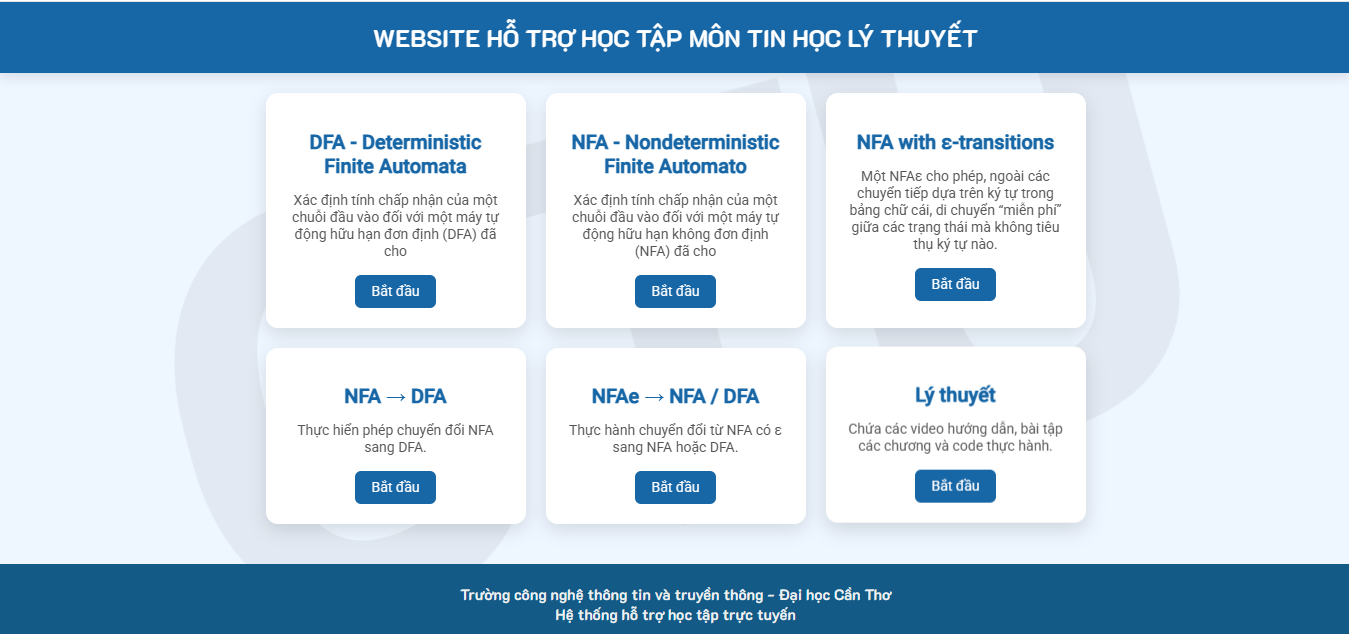
\includegraphics[width=\textwidth]{THLT_main.png}
    \caption{Giao diện chính của website}
    \label{fig:des_structure}
\end{figure}

\section{Chức năng kiểm tra DFA}

\begin{itemize}
    \item Cho phép người dùng \textbf{nhập một DFA} bao gồm:
    \begin{itemize}
        \item Tập trạng thái $Q$.
        \item Bảng chuyển trạng thái $\delta$.
        \item Trạng thái bắt đầu $q_0$.
        \item Tập trạng thái kết thúc $F$.
        \item Bảng ký hiệu đầu vào $\Sigma$.
    \end{itemize}
    \item Hỗ trợ \textbf{nhập chuỗi đầu vào} và kiểm tra xem chuỗi có được DFA chấp nhận hay không.
    \item Quá trình kiểm tra được \textbf{hiển thị từng bước}, làm nổi bật các trạng thái đang đi qua.
    \item Cung cấp \textbf{kết quả cuối cùng}: chuỗi được chấp nhận hay bị từ chối.
\end{itemize}

\begin{figure}[H]
    \centering
    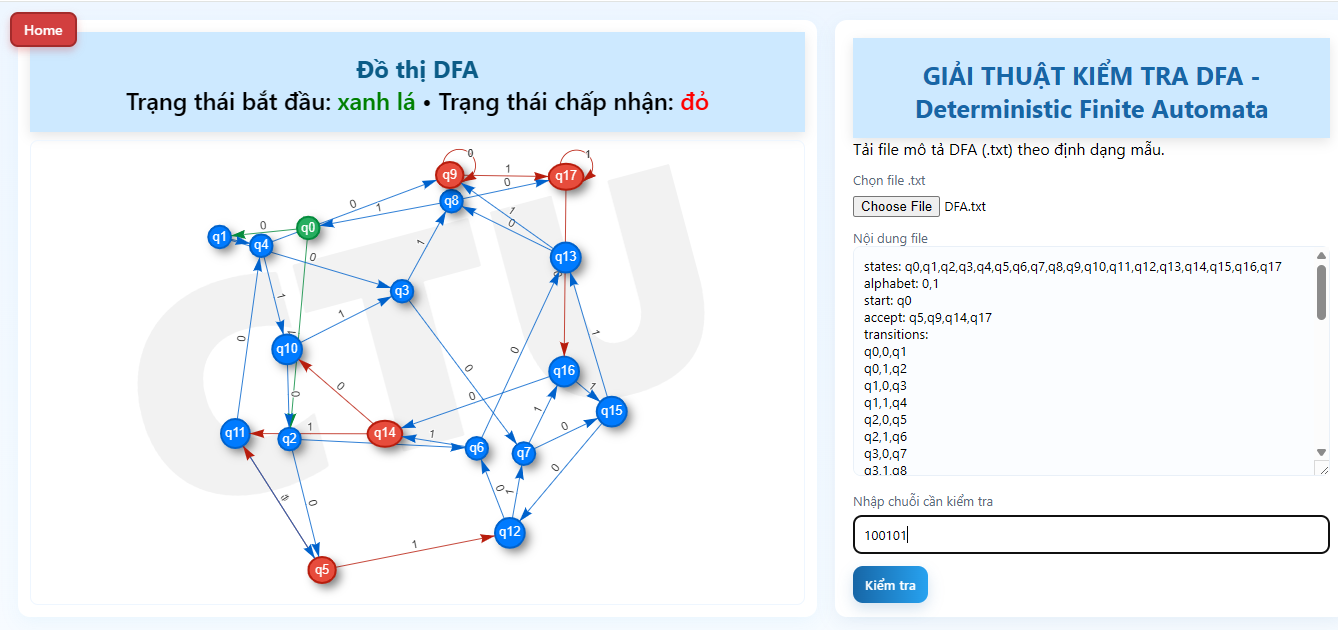
\includegraphics[width=\textwidth]{THLT_DFA.png}
    \caption{Giao diện trang kiểm tra DFA}
    \label{fig:des_structure}
\end{figure}
Hàm \texttt{simulateDFA(dfa, str)} dùng để mô phỏng cách một DFA xử lý một chuỗi ký tự. Nó bắt đầu bằng việc lấy trạng thái bắt đầu và khởi tạo các mảng lưu đường đi (\texttt{path}) và chi tiết từng bước (\texttt{details}), đồng thời tạo bảng chuyển $\delta$ để hiển thị. Nếu chuỗi rỗng, hàm kiểm tra ngay trạng thái bắt đầu có thuộc tập trạng thái chấp nhận hay không và trả kết quả. Nếu chuỗi không rỗng, hàm sẽ duyệt từng ký tự: với mỗi ký tự, nó tìm trạng thái tiếp theo theo bảng chuyển, lưu lại trạng thái hiện tại vào đường đi và chi tiết $\delta$ vào mảng \texttt{details}. Nếu gặp ký hiệu không có chuyển hợp lệ, hàm dừng và báo lỗi. Khi hết chuỗi, hàm kiểm tra trạng thái cuối cùng có thuộc tập \texttt{accept} hay không, tạo kết luận dạng LaTeX và trả về toàn bộ thông tin, bao gồm: kết quả chấp nhận/chối, đường đi các trạng thái, chi tiết từng bước và bảng $\delta$, phục vụ cho việc hiển thị trực quan trên giao diện.
\begin{algorithm}[H]
\caption{Mô phỏng một DFA với chuỗi đầu vào}
\begin{algorithmic}[1]
\Require DFA $M = (Q, \Sigma, \delta, q_0, F)$, chuỗi $w = w_1 w_2 \dots w_n$
\Ensure Xác định xem $w$ có được $M$ chấp nhận không và lưu lại các bước tính $\delta$
\State $cur \gets q_0$
\State $path \gets [q_0]$
\If{$w$ rỗng}
    \If{$q_0 \in F$}
        \State Kết luận: chuỗi rỗng được chấp nhận
    \Else
        \State Kết luận: chuỗi rỗng bị từ chối
    \EndIf
    \State \Return $path, \delta, kết luận$
\EndIf
\For{$i = 1$ \textbf{to} $n$}
    \State $sym \gets w_i$
    \If{$\delta(cur, sym)$ không xác định}
        \State Dừng: không có chuyển từ $cur$ với ký hiệu $sym$
        \State \Return thông báo lỗi và $path$ hiện tại
    \EndIf
    \State $cur \gets \delta(cur, sym)$
    \State Thêm $cur$ vào $path$
\EndFor
\If{$cur \in F$}
    \State Kết luận: chuỗi được chấp nhận
\Else
    \State Kết luận: chuỗi bị từ chối
\EndIf
\State \Return $path, \delta, kết luận$
\end{algorithmic}
\end{algorithm}


\section{Chức năng kiểm tra NFA}

\begin{itemize}
    \item Cho phép người dùng nhập một NFA với các thông tin tương tự DFA.
    \item Hỗ trợ kiểm tra chuỗi đầu vào \textbf{dựa trên tất cả các đường đi khả thi}.
    \item Giao diện hiển thị:
    \begin{itemize}
        \item Tất cả các đường đi đang được kiểm tra.
        \item Các trạng thái cuối cùng nếu chuỗi được chấp nhận.
    \end{itemize}
    \item Giúp sinh viên \textbf{quan sát đặc trưng phi định hướng của NFA}.
\end{itemize}
\begin{figure}[H]
    \centering
    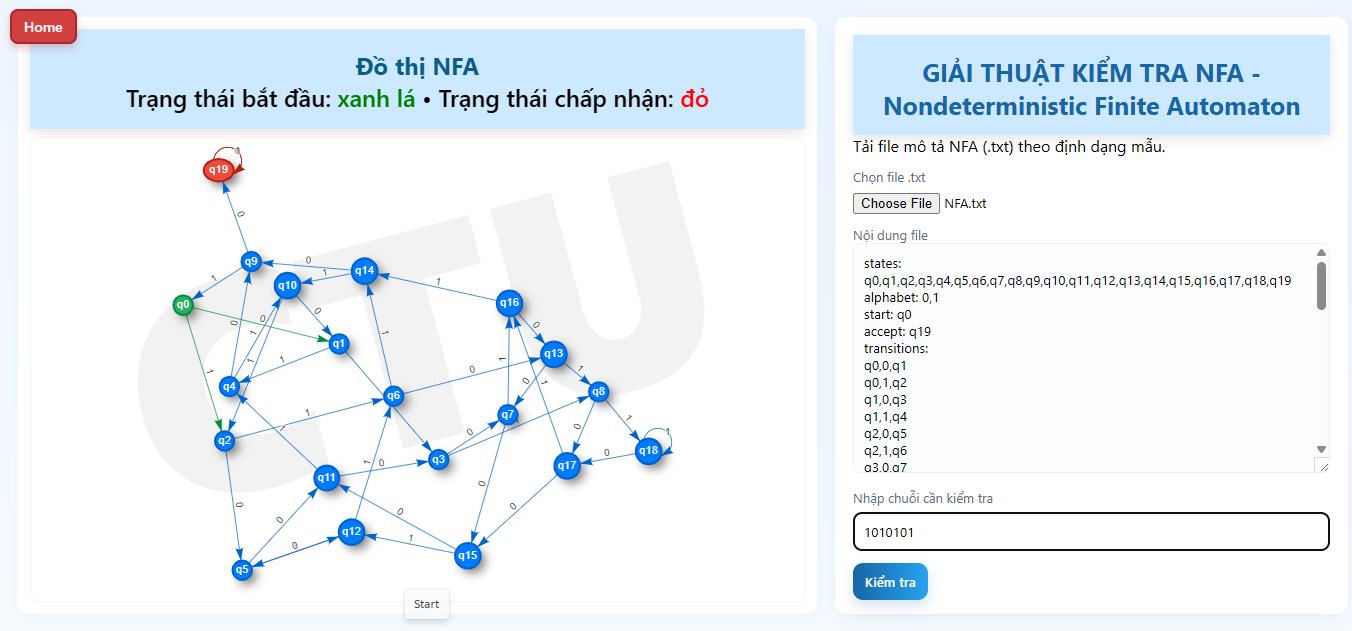
\includegraphics[width=\textwidth]{THLT_NFA.png}
    \caption{Giao diện trang kiểm tra NFA}
    \label{fig:des_structure}
\end{figure}

Hàm \texttt{simulateNFA(nfa, str)} dùng để mô phỏng cách một \textbf{NFA (Non-deterministic Finite Automaton)} xử lý một chuỗi ký tự. Nó bắt đầu bằng việc khởi tạo tập các trạng thái hiện tại (\texttt{currentStates}) chỉ chứa trạng thái bắt đầu, đồng thời tạo bảng chuyển $\delta$ (\texttt{deltaTable}) để hiển thị. Nếu chuỗi rỗng, hàm kiểm tra xem trạng thái bắt đầu có thuộc tập trạng thái chấp nhận hay không và tạo kết luận. Nếu chuỗi không rỗng, hàm duyệt từng ký tự trong chuỗi: với mỗi ký tự, nó xét tất cả các trạng thái hiện tại, tìm tất cả trạng thái đích mà NFA có thể chuyển tới, lưu tập các trạng thái này làm trạng thái hiện tại mới và ghi chi tiết bước vào mảng \texttt{details} dưới dạng biểu thức LaTeX. Nếu tại bất kỳ bước nào không còn trạng thái nào để chuyển, hàm dừng và báo lỗi. Khi hết chuỗi, hàm kiểm tra xem tập trạng thái cuối cùng có giao với tập trạng thái chấp nhận hay không để xác định chuỗi được chấp nhận hay bị từ chối, đồng thời trả về toàn bộ thông tin: kết quả, đường đi các tập trạng thái, chi tiết từng bước và bảng $\delta$, phục vụ hiển thị trực quan trên giao diện.
\begin{algorithm}[H]
\caption{Mô phỏng một NFA với chuỗi đầu vào}
\begin{algorithmic}[1]
\Require NFA $M = (Q, \Sigma, \delta, q_0, F)$, chuỗi $w = w_1 w_2 \dots w_n$
\Ensure Xác định xem $w$ có được NFA chấp nhận không và lưu lại các bước $\delta$
\State $currentStates \gets \{q_0\}$
\State $path \gets [currentStates]$

\If{$w$ rỗng}
    \If{$currentStates \cap F \neq \emptyset$}
        \State Kết luận: chuỗi rỗng được chấp nhận
    \Else
        \State Kết luận: chuỗi rỗng bị từ chối
    \EndIf
    \State \Return $path, \delta, kết luận$
\EndIf

\For{$i = 1$ \textbf{to} $n$}
    \State $sym \gets w_i$
    \State $nextStates \gets \emptyset$
    \For{mỗi $s$ trong $currentStates$}
        \If{$\delta(s, sym)$ tồn tại}
            \State $nextStates \gets nextStates \cup \delta(s, sym)$
        \EndIf
    \EndFor
    \State Ghi lại $\delta(currentStates, sym) = nextStates$ vào chi tiết
    \If{$nextStates = \emptyset$}
        \State Dừng: không có chuyển từ $currentStates$ với ký hiệu $sym$
        \State \Return thông báo lỗi và $path$ hiện tại
    \EndIf
    \State $currentStates \gets nextStates$
    \State Thêm $currentStates$ vào $path$
\EndFor

\If{$currentStates \cap F \neq \emptyset$}
    \State Kết luận: chuỗi được chấp nhận
\Else
    \State Kết luận: chuỗi bị từ chối
\EndIf
\State \Return $path, \delta, kết luận$
\end{algorithmic}
\end{algorithm}

\section{Chức năng kiểm tra NFA$\epsilon$}

\begin{itemize}
    \item Nhập NFA$\epsilon$ với các mũi tên $\epsilon$.
    \item Tự động tính \textbf{epsilon-closure} của từng trạng thái.
    \item Cho phép kiểm tra chuỗi đầu vào tương tự NFA.
    \item Giao diện trực quan hiển thị:
    \begin{itemize}
        \item Các bước epsilon-closure.
        \item Đường đi khả thi theo chuỗi đầu vào.
    \end{itemize}
\end{itemize}
\begin{figure}[H]
    \centering
    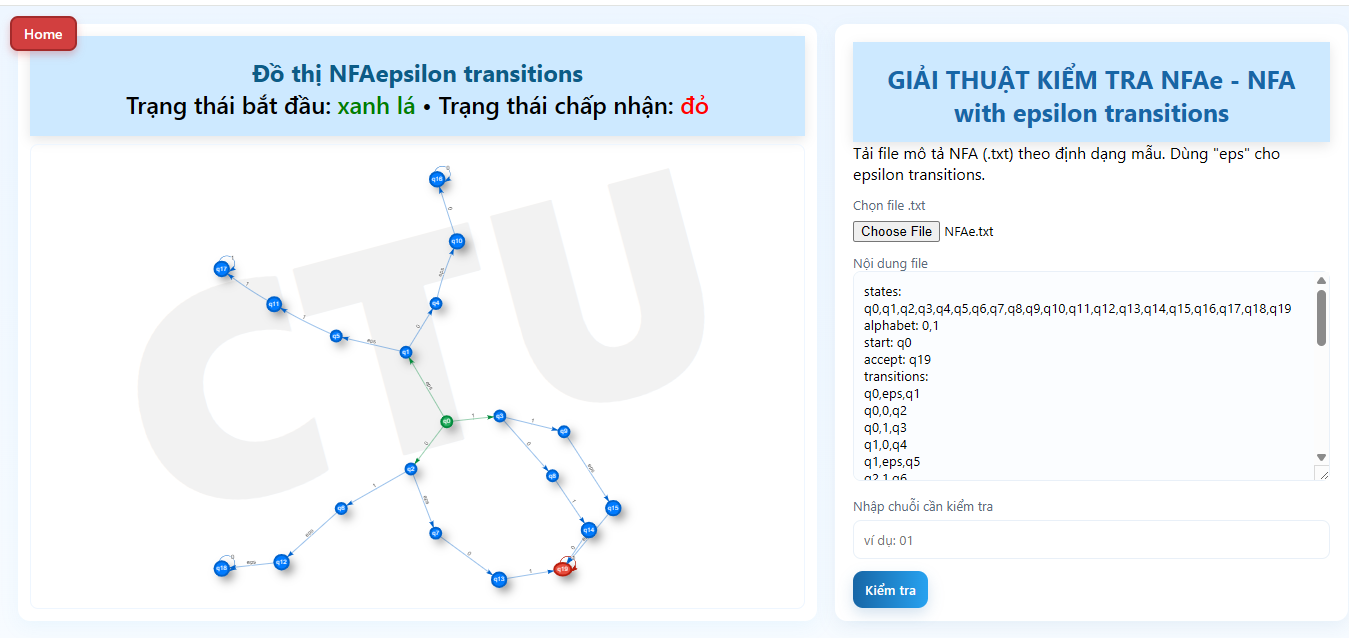
\includegraphics[width=\textwidth]{THLT_NFAe.png}
    \caption{Giao diện trang kiểm tra NFAe}
    \label{fig:des_structure}
\end{figure}

Hàm \texttt{simulateNFAe(nfa, str)} được sử dụng để mô phỏng việc NFA xử lý một chuỗi ký tự có thể chứa epsilon. Khi bắt đầu, hàm lấy trạng thái bắt đầu của NFA và khởi tạo các tập trạng thái hiện tại (\texttt{currentStates}), mảng lưu đường đi (\texttt{path}) và chi tiết từng bước (\texttt{details}). Hàm \texttt{statesToTex} được định nghĩa để chuyển các tập trạng thái thành biểu diễn LaTeX, phục vụ hiển thị trực quan.

Nếu chuỗi nhập vào rỗng, hàm ngay lập tức kiểm tra xem trạng thái bắt đầu có thuộc tập trạng thái chấp nhận hay không và tạo kết luận tương ứng, đồng thời ghi chi tiết vào mảng \texttt{details}.  

Nếu chuỗi không rỗng, hàm duyệt từng ký tự trong chuỗi. Với mỗi ký tự, hàm tạo một tập trạng thái tiếp theo (\texttt{nextStates}) bằng cách duyệt các trạng thái hiện tại và tìm các chuyển hợp lệ theo bảng chuyển \(\delta\) của NFA. Sau đó, biểu diễn các bước chuyển được ghi vào \texttt{details}. Nếu tại bước nào không có chuyển hợp lệ, hàm dừng và trả về thông báo lỗi cùng chi tiết các bước đã thực hiện.  

Khi hết chuỗi, hàm kiểm tra xem tập trạng thái cuối cùng có chứa ít nhất một trạng thái chấp nhận hay không, tạo kết luận về việc chuỗi được chấp nhận hay bị từ chối, và trả về một đối tượng gồm: trạng thái chấp nhận/chối, đường đi qua các trạng thái, chi tiết từng bước và bảng \(\delta\), phục vụ cho việc hiển thị trực quan trên giao diện. Như vậy, hàm này cung cấp cơ chế mô phỏng NFA một cách chi tiết, đồng thời hỗ trợ trực quan hóa các bước xử lý chuỗi với epsilon.
\begin{algorithm}[H]
\caption{Mô phỏng một $\epsilon$-NFA với chuỗi đầu vào}
\begin{algorithmic}[1]
\Require $\epsilon$-NFA $M = (Q, \Sigma, \delta, q_0, F)$, chuỗi $w = w_1 w_2 \dots w_n$
\Ensure Xác định xem $w$ có được NFA chấp nhận không và lưu lại các bước $\delta$
\State $currentStates \gets \epsilon\text{-closure}(\{q_0\})$
\State $path \gets [currentStates]$

\If{$w$ rỗng}
    \If{$currentStates \cap F \neq \emptyset$}
        \State Kết luận: chuỗi rỗng được chấp nhận
    \Else
        \State Kết luận: chuỗi rỗng bị từ chối
    \EndIf
    \State \Return $path, \delta, kết luận$
\EndIf

\For{$i = 1$ \textbf{to} $n$}
    \State $sym \gets w_i$
    \State $nextStates \gets \emptyset$
    \For{mỗi $s$ trong $currentStates$}
        \If{$\delta(s, sym)$ tồn tại}
            \State $nextStates \gets nextStates \cup \delta(s, sym)$
        \EndIf
    \EndFor
    \State Ghi lại $\delta(currentStates, sym) = nextStates$ vào chi tiết
    \If{$nextStates = \emptyset$}
        \State Dừng: không có chuyển từ $currentStates$ với ký hiệu $sym$
        \State \Return thông báo lỗi và $path$ hiện tại
    \EndIf
    \State $currentStates \gets \epsilon\text{-closure}(nextStates)$
    \State Thêm $currentStates$ vào $path$
\EndFor

\If{$currentStates \cap F \neq \emptyset$}
    \State Kết luận: chuỗi được chấp nhận
\Else
    \State Kết luận: chuỗi bị từ chối
\EndIf
\State \Return $path, \delta, kết luận$
\end{algorithmic}
\end{algorithm}

\section{Chức năng chuyển NFA sang DFA}

\begin{itemize}
    \item Sử dụng \textbf{thuật toán xây dựng tập con (subset construction)} để chuyển đổi.
    \item Mỗi trạng thái DFA tương ứng với một tập con trạng thái NFA.
    \item Giao diện hiển thị:
    \begin{itemize}
        \item Bảng chuyển trạng thái DFA.
        \item Sơ đồ trạng thái trực quan.
        \item Liên kết từng trạng thái DFA với tập con NFA tương ứng.
    \end{itemize}
\end{itemize}
\begin{figure}[H]
    \centering
    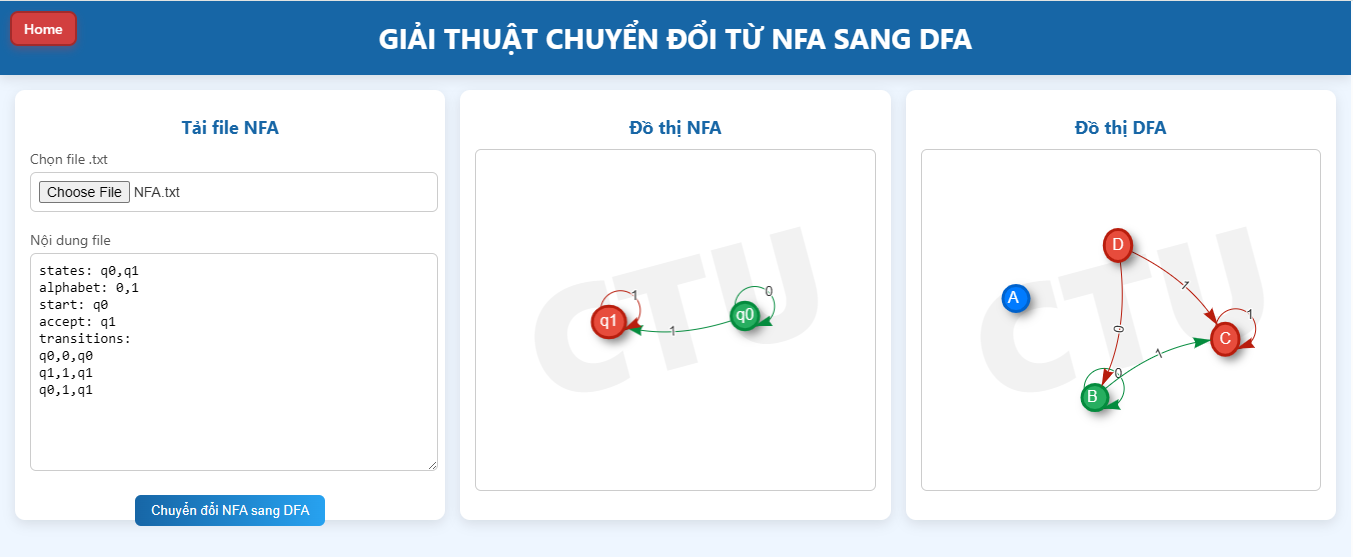
\includegraphics[width=\textwidth]{THLT_NFADFA.png}
    \caption{Giao diện chức năng chuyển NFA sang DFA}
    \label{fig:des_structure}
\end{figure}

Hàm \texttt{convertNFAtoDFA(nfa, callback)} thực hiện việc chuyển đổi một NFA sang DFA. Trước tiên, hàm tạo tất cả các tập con có thể của tập trạng thái NFA, mỗi tập con sẽ đại diện cho một trạng thái tiềm năng của DFA. Mỗi tập con được gán một tên duy nhất dựa trên ký tự chữ cái (A, B, C, ...). Sau đó, hàm xây dựng bảng chuyển đổi của DFA (\texttt{dfaTrans}) bằng cách duyệt qua từng tập con và từng ký hiệu trong bảng chữ cái (trừ ký hiệu epsilon). Với mỗi trạng thái NFA trong tập con, nếu tồn tại chuyển với ký hiệu hiện tại, hàm sẽ tính epsilon-closure của trạng thái đích và gộp vào tập trạng thái tiếp theo của DFA. Nếu tập trạng thái tiếp theo không rỗng, nó sẽ được ghi vào bảng chuyển và gọi hàm \texttt{callback} để lưu chi tiết bước chuyển đổi, phục vụ hiển thị trực quan. Trạng thái bắt đầu của DFA được xác định là epsilon-closure của trạng thái bắt đầu NFA, và tập trạng thái chấp nhận của DFA gồm tất cả các tập con chứa ít nhất một trạng thái chấp nhận của NFA. Cuối cùng, hàm trả về đối tượng DFA bao gồm tập trạng thái, bảng chữ cái (loại trừ epsilon), trạng thái bắt đầu, tập trạng thái chấp nhận và bảng chuyển. Như vậy, hàm này cung cấp cơ chế chuyển đổi toàn diện từ NFA sang DFA, đồng thời cho phép quan sát chi tiết quá trình xây dựng thông qua callback.  

\begin{algorithm}[H]
\caption{Chuyển NFAsang DFA bằng thuật toán tập con (Subset Construction)}
\begin{algorithmic}[1]
\Require NFA $M = (Q, \Sigma, \delta, q_0, F)$
\Ensure DFA $M' = (Q', \Sigma', \delta', q_0', F')$
\State $allStates \gets Q$
\State $subsets \gets \text{tập tất cả tập con của } Q$

\Comment{Gán tên cho các tập con DFA}
\State $stateNames \gets$ rỗng
\State $nameCharCode \gets 65$ \Comment{dùng A, B, C, ...}
\For{mỗi $subset$ trong $subsets$}
    \State $key \gets \text{chuỗi các trạng thái trong subset, sắp xếp theo thứ tự}$
    \State $stateNames[key] \gets \text{ký tự tiếp theo từ nameCharCode}$
    \State tăng $nameCharCode$
\EndFor

\Comment{Xây dựng bảng chuyển trạng thái DFA}
\State $dfaTrans \gets$ rỗng
\For{mỗi $subset$ trong $subsets$}
    \State $dfaStateName \gets stateNames[subset]$
    \For{mỗi $sym$ trong $\Sigma \setminus \{\epsilon\}$}
        \State $nextSet \gets \emptyset$
        \For{mỗi $s$ trong $subset$}
            \If{$\delta(s, sym)$ tồn tại}
                \For{mỗi $t \in \delta(s, sym)$}
                    \State $nextSet \gets nextSet \cup \epsilon\text{-closure}(\{t\})$
                \EndFor
            \EndIf
        \EndFor
        \If{$nextSet \neq \emptyset$}
            \State $nextKey \gets$ chuỗi các trạng thái trong $nextSet$ sắp xếp theo thứ tự
            \State $dfaTrans[dfaStateName][sym] \gets stateNames[nextKey]$
        \EndIf
    \EndFor
\EndFor

\Comment{Xác định trạng thái bắt đầu và trạng thái kết thúc của DFA}
\State $startClosure \gets \epsilon\text{-closure}(\{q_0\})$
\State $q_0' \gets stateNames[startClosure]$
\State $F' \gets \{ stateNames[subset] \mid subset \cap F \neq \emptyset \}$

\State \Return DFA $M' = (Q', \Sigma', \delta', q_0', F')$
\end{algorithmic}
\end{algorithm}

\section{Chức năng chuyển NFA$\epsilon$ sang DFA hoặc NFA}

\begin{itemize}
    \item Hỗ trợ hai dạng chuyển đổi:
    \begin{enumerate}
        \item NFA$\epsilon \rightarrow$ NFA: loại bỏ các mũi tên $\epsilon$ thông qua epsilon-closure.
        \item NFA$\epsilon \rightarrow$ DFA: kết hợp epsilon-closure và subset construction.
    \end{enumerate}
    \item Giao diện trực quan:
    \begin{itemize}
        \item Hiển thị sơ đồ NFA$\epsilon$ ban đầu.
        \item Hiển thị NFA hoặc DFA kết quả, có mũi tên nối từ trạng thái cũ sang trạng thái mới.
        \item Hiển thị bảng chuyển trạng thái chi tiết.
    \end{itemize}
\end{itemize}
\begin{figure}[H]
    \centering
    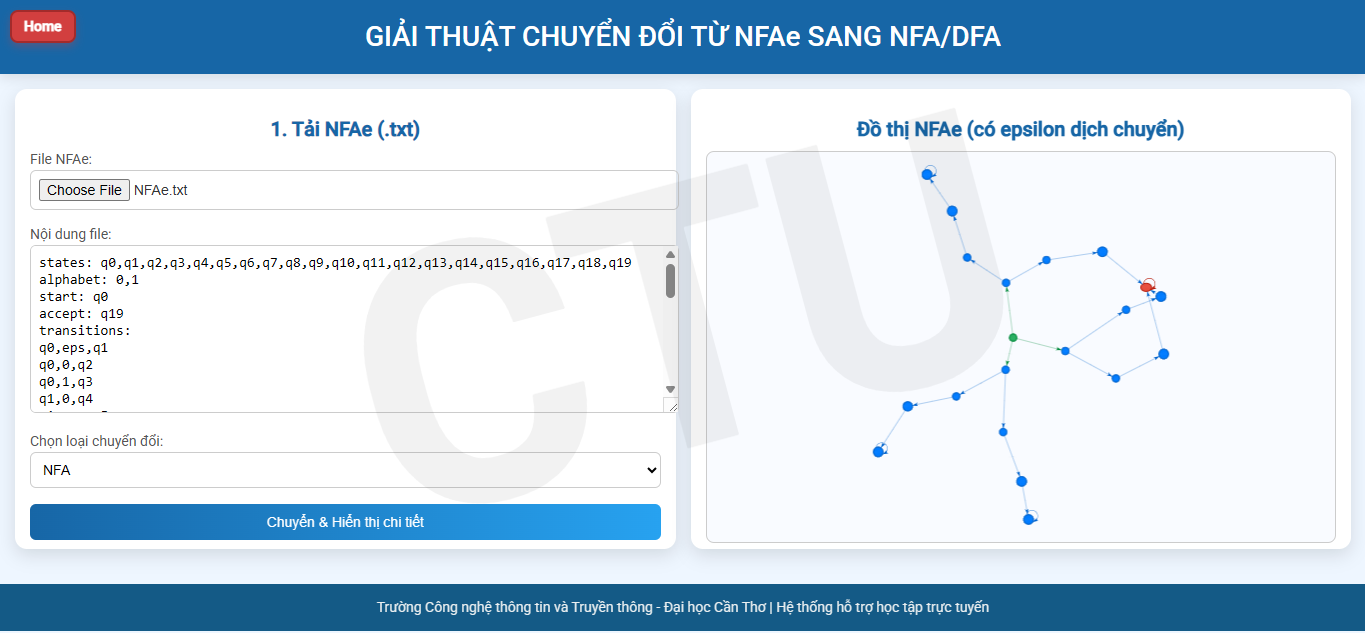
\includegraphics[width=\textwidth]{THLT_NFAeNFADFA.png}
    \caption{Giao diện chức năng chuyển NFAe sang NFA hoặc DFA}
    \label{fig:des_structure}
\end{figure}

Hàm \texttt{epsilonClosure(nfae, states)} được sử dụng để tính \emph{epsilon-closure} của một tập trạng thái trong NFA có epsilon (NFA\(\epsilon\)). Khi được gọi, hàm bắt đầu với một ngăn xếp (\texttt{stack}) chứa tất cả các trạng thái trong tập \texttt{states} và một tập \texttt{closure} cũng bao gồm các trạng thái này.  

Trong vòng lặp \texttt{while}, hàm lấy ra từng trạng thái từ ngăn xếp và kiểm tra xem từ trạng thái đó có các chuyển \(\epsilon\) hay không. Nếu tồn tại, mỗi trạng thái đích của chuyển \(\epsilon\) sẽ được thêm vào tập \texttt{closure} nếu chưa có, đồng thời được đẩy vào ngăn xếp để tiếp tục kiểm tra các chuyển \(\epsilon\) tiếp theo.  

Quá trình này tiếp tục cho đến khi không còn trạng thái nào trong ngăn xếp, đảm bảo rằng tất cả các trạng thái có thể đạt được từ tập trạng thái ban đầu thông qua các chuyển \(\epsilon\) đều được bao gồm trong \texttt{closure}. Cuối cùng, hàm trả về tập \texttt{closure} này, cho phép sử dụng trong việc chuyển đổi NFA sang DFA hoặc mô phỏng NFA.
\begin{algorithm}[H]
\caption{Tính $\epsilon$-closure của một tập trạng thái trong NFA$\epsilon$}
\begin{algorithmic}[1]
\Require NFA$\epsilon$ $M = (Q, \Sigma, \delta, q_0, F)$, tập trạng thái $S \subseteq Q$
\Ensure $\epsilon$-closure của $S$
\State $stack \gets S$
\State $closure \gets S$
\While{$stack \neq \emptyset$}
    \State $s \gets stack.pop()$
    \If{$\delta(s, \epsilon)$ tồn tại}
        \For{mỗi trạng thái $t \in \delta(s, \epsilon)$}
            \If{$t \notin closure$}
                \State $closure \gets closure \cup \{t\}$
                \State $stack.push(t)$
            \EndIf
        \EndFor
    \EndIf
\EndWhile
\State \Return $closure$
\end{algorithmic}
\end{algorithm}


Hàm \texttt{convertNFAeToNFA(nfae)} được sử dụng để chuyển một NFA có epsilon (\(\epsilon\)-NFA) thành một NFA thông thường (không có epsilon). Đầu tiên, hàm tạo một đối tượng \texttt{newTrans} để lưu các bảng chuyển mới. Với mỗi trạng thái \texttt{s} trong NFA gốc, hàm duyệt qua từng ký hiệu trong bảng chữ cái (ngoại trừ \(\epsilon\)).  

Đối với mỗi ký hiệu, hàm tính \emph{epsilon-closure} của trạng thái \texttt{s} (\texttt{eps\_s}) để xác định tất cả các trạng thái có thể đạt được từ \texttt{s} chỉ bằng các chuyển \(\epsilon\). Sau đó, với mỗi trạng thái \texttt{q} trong \texttt{eps\_s}, nếu có chuyển ký hiệu hiện tại từ \texttt{q} đến trạng thái \texttt{r}, hàm tiếp tục lấy \emph{epsilon-closure} của \texttt{r} và thêm tất cả các trạng thái này vào tập đích \texttt{dstSet}. Nếu tập này không rỗng, nó được lưu trong bảng chuyển \texttt{newTrans} cho trạng thái \texttt{s} và ký hiệu hiện tại.  

Tiếp theo, hàm xác định tập trạng thái chấp nhận mới \texttt{newAccept} bằng cách thêm các trạng thái \texttt{s} nếu \emph{epsilon-closure} của \texttt{s} chứa ít nhất một trạng thái chấp nhận của NFA gốc.  

Cuối cùng, hàm trả về một NFA mới với các thuộc tính: tập trạng thái (\texttt{states}) giữ nguyên, bảng chữ cái loại bỏ ký hiệu \(\epsilon\), trạng thái bắt đầu (\texttt{start}) giữ nguyên, tập trạng thái chấp nhận mới (\texttt{accept}) và bảng chuyển mới (\texttt{transitions}), đảm bảo rằng NFA thu được có cùng ngôn ngữ với \(\epsilon\)-NFA ban đầu nhưng không còn epsilon transitions.

\begin{algorithm}[H]
\caption{Chuyển NFA$\epsilon$ sang NFA}
\begin{algorithmic}[1]
\Require NFA$\epsilon$ $M = (Q, \Sigma, \delta, q_0, F)$
\Ensure NFA $M' = (Q, \Sigma', \delta', q_0, F')$
\State $Q' \gets Q$
\State $\Sigma' \gets \Sigma \setminus \{\epsilon\}$
\State $\delta' \gets$ rỗng

\For{mỗi trạng thái $s \in Q$}
    \For{mỗi ký hiệu $a \in \Sigma'$}
        \State $dstSet \gets \emptyset$
        \State $eps_s \gets \epsilon\text{-closure}(\{s\})$
        \For{mỗi trạng thái $q \in eps_s$}
            \If{$\delta(q, a)$ tồn tại}
                \For{mỗi $r \in \delta(q, a)$}
                    \State $dstSet \gets dstSet \cup \epsilon\text{-closure}(\{r\})$
                \EndFor
            \EndIf
        \EndFor
        \If{$dstSet \neq \emptyset$}
            \State $\delta'(s, a) \gets dstSet$
        \EndIf
    \EndFor
\EndFor

\State $F' \gets \{ s \in Q \mid \epsilon\text{-closure}(\{s\}) \cap F \neq \emptyset \}$
\State \Return NFA $M' = (Q', \Sigma', \delta', q_0, F')$
\end{algorithmic}
\end{algorithm}



Hàm \texttt{convertNFAtoDFA(nfa, callback)} thực hiện việc chuyển một NFA (có thể có epsilon transitions) sang DFA. Ban đầu, hàm tính \emph{epsilon-closure} của trạng thái bắt đầu NFA để tạo trạng thái bắt đầu của DFA và đánh dấu nó là chưa xử lý. Tên các trạng thái DFA được gán tuần tự từ 'A', 'B', ... dựa trên tập hợp các trạng thái NFA hợp thành.

Trong quá trình lặp, hàm lấy từng trạng thái chưa đánh dấu, duyệt qua tất cả các ký hiệu của bảng chữ cái (ngoại trừ \(\epsilon\)), và tính tập trạng thái tiếp theo bằng cách áp dụng các chuyển từ trạng thái hiện tại theo ký hiệu và \emph{epsilon-closure}. Nếu tập trạng thái tiếp theo chưa được đặt tên, hàm sẽ tạo tên mới và thêm vào danh sách các trạng thái chưa đánh dấu. Đồng thời, hàm lưu các bước chuyển đổi và gọi \texttt{callback} nếu được cung cấp, giúp theo dõi quá trình chuyển đổi.

Sau khi xử lý hết các trạng thái, hàm xây dựng đối tượng DFA cuối cùng với các thuộc tính: tập trạng thái (\texttt{states}), bảng chữ cái (\texttt{alphabet}) loại bỏ \(\epsilon\), trạng thái bắt đầu ('A'), tập trạng thái chấp nhận (\texttt{accept}) bao gồm tất cả các trạng thái DFA chứa ít nhất một trạng thái chấp nhận của NFA ban đầu, và bảng chuyển (\texttt{transitions}) từ tên trạng thái DFA theo ký hiệu. DFA thu được đảm bảo nhận cùng ngôn ngữ với NFA gốc nhưng không còn epsilon transitions và mỗi ký hiệu dẫn đến đúng một trạng thái tiếp theo.
\begin{algorithm}[H]
\caption{Chuyển NFA sang DFA bằng thuật toán tập con}
\begin{algorithmic}[1]
\Require NFA $M = (Q, \Sigma, \delta, q_0, F)$
\Ensure DFA $M' = (Q', \Sigma, \delta', q_0', F')$
\State $startClosure \gets \epsilon\text{-closure}(\{q_0\})$
\State $unmarked \gets [startClosure]$
\State $stateNames[startClosure] \gets 'A'$
\State $nameCharCode \gets 66$
\State $dfaTrans \gets$ rỗng

\While{$unmarked \neq \emptyset$}
    \State $curr \gets unmarked.shift()$
    \State $currName \gets stateNames[curr]$
    \For{mỗi $sym \in \Sigma \setminus \{\epsilon\}$}
        \State $nextSet \gets \emptyset$
        \For{mỗi $s \in curr$}
            \If{$\delta(s, sym)$ tồn tại}
                \For{mỗi $t \in \delta(s, sym)$}
                    \State $nextSet \gets nextSet \cup \epsilon\text{-closure}(\{t\})$
                \EndFor
            \EndIf
        \EndFor
        \If{$nextSet \neq \emptyset$}
            \If{$stateNames[nextSet]$ chưa tồn tại}
                \State $stateNames[nextSet] \gets \text{ký tự tiếp theo từ nameCharCode}$
                \State tăng $nameCharCode$
            \EndIf
            \State $dfaTrans[currName][sym] \gets stateNames[nextSet]$
            \If{$nextSet$ chưa được đánh dấu} 
                \State thêm $nextSet$ vào $unmarked$
            \EndIf
        \EndIf
    \EndFor
\EndWhile

\State $Q' \gets \text{tập các giá trị trong stateNames}$
\State $q_0' \gets stateNames[startClosure]$
\State $F' \gets \{ stateNames[subset] \mid subset \cap F \neq \emptyset \}$
\State \Return DFA $M' = (Q', \Sigma, \delta', q_0', F')$
\end{algorithmic}
\end{algorithm}


\section{Chức năng lý thuyết và bài tập}
\hspace*{0.7cm}Tài liệu này cung cấp lý thuyết đầy đủ về các mô hình tự động hữu hạn, bao gồm DFA, NFA và NFA$\epsilon$, nhằm giúp học sinh nắm vững khái niệm cơ bản về cách các tự động hoạt động và biểu diễn các ngôn ngữ chính thức. Bên cạnh việc học các thuật toán chuyển đổi giữa các mô hình, sinh viên còn được hướng dẫn cách xác định epsilon-closure và thực hiện subset construction để xây dựng các tự động tương đương, từ đó hình thành tư duy hệ thống trong việc phân tích và thiết kế các mô hình.  
\begin{figure}[H]
    \centering
    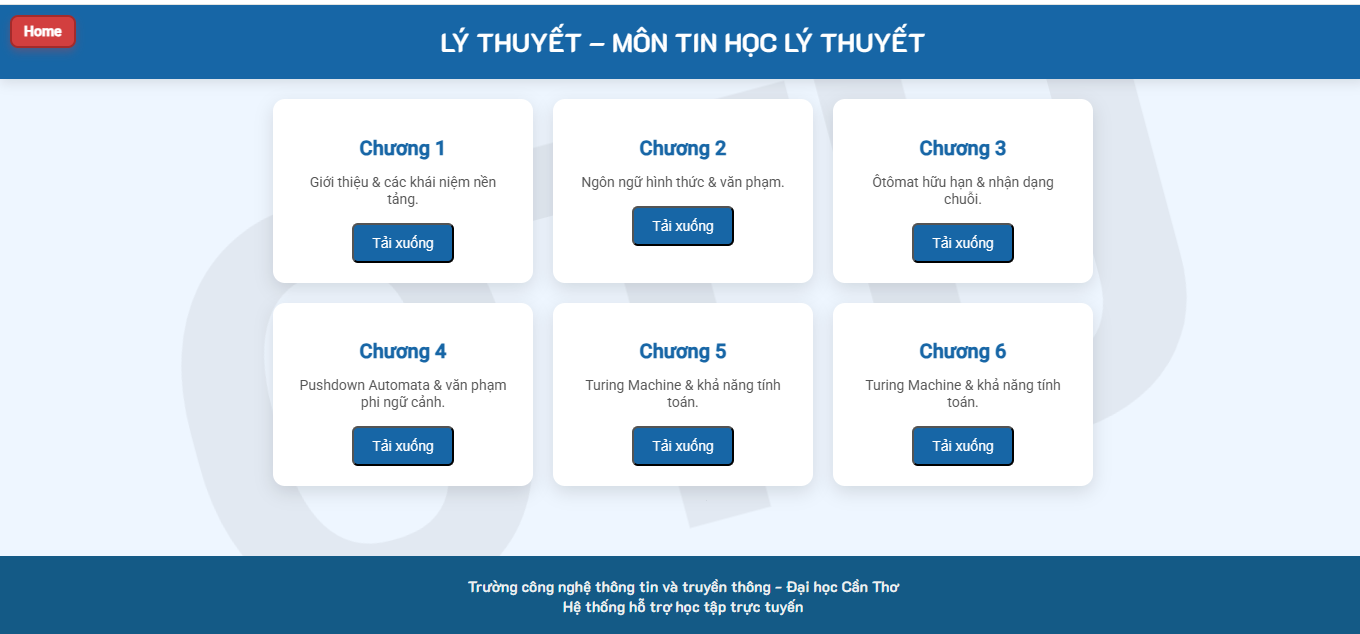
\includegraphics[width=\textwidth]{THLT_LT.png}
    \caption{Giao diện chức năng cung cấp lý thuyết}
    \label{fig:des_structure}
\end{figure}

Ngoài phần lý thuyết, tài liệu cũng chia sẻ kinh nghiệm làm bài tập tự giải: các ví dụ minh họa từng bước cách kiểm tra chuỗi đầu vào, cách chuyển đổi từ NFA sang DFA, và cách tính toán tập epsilon-closure cho từng trạng thái. Việc thực hành này giúp học sinh tự đánh giá năng lực, rèn luyện kỹ năng tư duy trừu tượng và tăng khả năng giải quyết các bài tập khó trong SGK cũng như các bài tập ôn trên lớp. Nhờ đó, sinh viên không chỉ học thuộc lý thuyết mà còn biết cách áp dụng vào các tình huống thực tế, hình thành thói quen tự học và tự kiểm tra hiệu quả.


\begin{figure}[H]
    \centering
    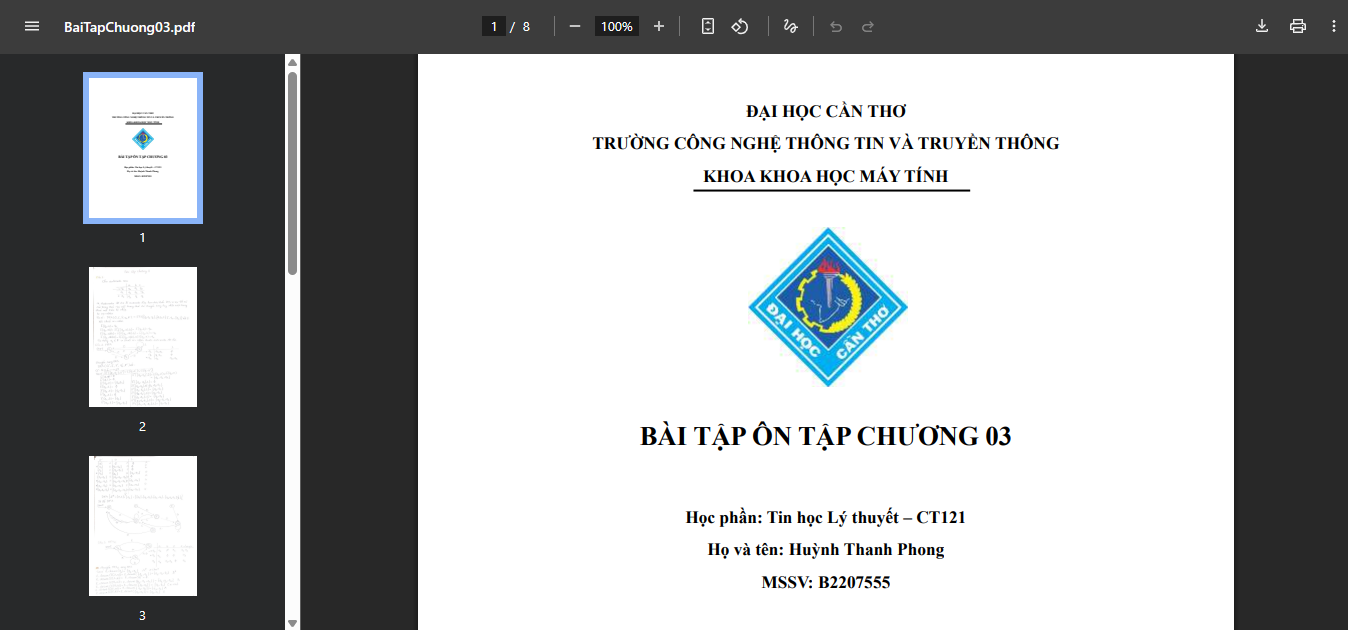
\includegraphics[width=\textwidth]{THLT_BT.png}
    \caption{Giao diện lý thuyết được hiển thị}
    \label{fig:des_structure}
\end{figure}
\chapter{TỔNG KẾT VÀ ĐÁNH GIÁ HƯỚNG PHÁT TRIỂN}

\section{Ưu điểm của hệ thống}
\hspace*{0.7cm}Hệ thống website hỗ trợ học tập môn \emph{Tin học lý thuyết} được xây dựng nhằm cung cấp môi trường học tập trực quan, sinh động và dễ sử dụng cho sinh viên. Một số ưu điểm chính gồm:

\begin{itemize}
    \item \textbf{Giao diện trực quan và sinh động:} Hệ thống hiển thị các trạng thái, mũi tên chuyển đổi, bảng chuyển trạng thái chi tiết và các bước epsilon-closure hay subset construction, giúp sinh viên quan sát trực tiếp quá trình hoạt động của DFA, NFA và NFA$\epsilon$.
    \item \textbf{Tích hợp lý thuyết và thực hành:} Phần lý thuyết đi kèm bài tập minh họa giúp sinh viên vừa học lý thuyết vừa thực hành trực tiếp, kiểm tra kết quả và củng cố kiến thức.
    \item \textbf{Kiểm tra chuỗi chi tiết:} Chức năng kiểm tra chuỗi hiển thị từng bước chuyển trạng thái, làm nổi bật trạng thái đang đi qua, giúp sinh viên dễ dàng theo dõi và nắm bắt cơ chế hoạt động của ôtômát.
    \item \textbf{Minh họa thuật toán chuyển đổi:} Các thuật toán chuyển NFA sang DFA và NFA$\epsilon$ sang NFA/DFA được trình bày trực quan, giúp sinh viên dễ hình dung mối quan hệ giữa các tập trạng thái.
    \item \textbf{Công nghệ hiện đại:} Sử dụng HTML5, CSS3, JavaScript, Bootstrap, Node.js/Servlets và thư viện vẽ đồ thị, giúp hệ thống hoạt động mượt mà, dễ dàng mở rộng và bảo trì.
    \item \textbf{Tùy chọn lưu trữ linh hoạt:} Hệ thống hỗ trợ lưu trữ dữ liệu ôtômát qua LocalStorage hoặc cơ sở dữ liệu MySQL/MongoDB, mang lại trải nghiệm học tập linh hoạt và trực quan.
\end{itemize}

\section{Hạn chế của hệ thống}
Mặc dù hệ thống đã đạt được mục tiêu cơ bản, vẫn tồn tại một số hạn chế cần khắc phục trong các phiên bản tiếp theo:

\begin{itemize}
    \item \textbf{Hiệu năng với ôtômát lớn:} Khi nhập các NFA$\epsilon$ phức tạp với nhiều trạng thái và epsilon-closure, hệ thống trên trình duyệt đôi khi chạy chậm do giới hạn tài nguyên.
    \item \textbf{Chưa có tạo bài tập tự động:} Hệ thống chưa hỗ trợ sinh ngẫu nhiên bài tập kiểm tra DFA/NFA/NFA$\epsilon$, dẫn đến việc sinh viên phải tự tạo bài tập thủ công.
    \item \textbf{Thiếu thống kê tiến độ học tập:} Chưa có chức năng lưu lịch sử thực hành, theo dõi điểm số hay thời gian thực hành, khiến giảng viên khó đánh giá kết quả học tập sinh viên.
    \item \textbf{Chưa tối ưu cho thiết bị di động:} Giao diện chưa hoàn toàn responsive, chưa tối ưu trải nghiệm trên màn hình nhỏ hoặc cảm ứng.
    \item \textbf{Hạn chế trong chia sẻ dữ liệu:} Hệ thống hiện chỉ lưu trữ cục bộ, chưa có tính năng chia sẻ ôtômát và kết quả thực hành trực tuyến giữa nhiều người dùng.
\end{itemize}

\section{Hướng phát triển}
\hspace*{0.7cm}Dựa trên các ưu điểm và hạn chế, hệ thống có thể phát triển theo các hướng sau để nâng cao hiệu quả học tập và trải nghiệm người dùng:

\begin{itemize}
    \item \textbf{Tối ưu hóa hiệu năng:} Sử dụng các thuật toán tối ưu, hoặc tích hợp WebAssembly để xử lý các ôtômát lớn, giảm độ trễ khi kiểm tra chuỗi và chuyển đổi trạng thái.
    \item \textbf{Sinh bài tập tự động:} Thêm chức năng tạo ngẫu nhiên bài tập kiểm tra DFA, NFA, NFA$\epsilon$ theo mức độ khó hoặc dựa trên tiến độ học tập của sinh viên.
    \item \textbf{Thống kê và báo cáo học tập:} Lưu trữ kết quả thực hành, theo dõi tiến độ học tập, số lần kiểm tra và điểm số, giúp giảng viên đánh giá và hướng dẫn sinh viên hiệu quả hơn.
    \item \textbf{Hỗ trợ mô hình nâng cao:} Mở rộng sang các mô hình ôtômát phức tạp hơn như Pushdown Automata (PDA) hoặc Turing Machine, phục vụ nghiên cứu nâng cao.
    \item \textbf{Cải thiện giao diện đa nền tảng:} Thiết kế responsive hoàn toàn, hỗ trợ màn hình nhỏ, cảm ứng và thêm hiệu ứng trực quan sinh động.
    \item \textbf{Lưu trữ và chia sẻ dữ liệu trực tuyến:} Kết nối hệ thống với cơ sở dữ liệu đám mây, cho phép sinh viên lưu trữ, chia sẻ ôtômát và kết quả thực hành.
    \item \textbf{Mở rộng phần lý thuyết và bài tập:} Tích hợp thêm các bài tập tự đánh giá, bài tập theo nhóm hoặc chế độ thi thử trực tuyến, tăng cường tương tác và đánh giá kiến thức.
\end{itemize}

\textbf{Kết luận}
Hệ thống đã đạt được mục tiêu cơ bản trong việc hỗ trợ học tập môn \emph{Tin học lý thuyết}, tạo môi trường học tập trực quan, tương tác và sinh động. Các ưu điểm giúp sinh viên nắm vững kiến thức về ôtômát, trong khi các hạn chế và hướng phát triển đã chỉ ra những điểm cần cải tiến trong các phiên bản tiếp theo, nhằm nâng cao hiệu quả giảng dạy và trải nghiệm người dùng.


\begin{thebibliography}{99}

% ---------------- TIẾNG ANH ----------------
\bibitem{sipser}
Michael Sipser, \textit{Introduction to the Theory of Computation}, 3rd Edition, Cengage Learning, 2012.

\bibitem{hopcroft}
John E. Hopcroft, Rajeev Motwani, Jeffrey D. Ullman,
\textit{Automata Theory, Languages, and Computation}, 3rd Edition, Pearson, 2007.

\bibitem{linz}
Peter Linz, \textit{An Introduction to Formal Languages and Automata}, 6th Edition, Jones \& Bartlett Learning, 2016.

\bibitem{lewis_papadimitriou}
Harry R. Lewis and Christos H. Papadimitriou,
\textit{Elements of the Theory of Computation}, 2nd Edition, Prentice Hall, 1997.

% ---------------- TIẾNG VIỆT ----------------
\bibitem{nguyenthithanh}
Nguyễn Thị Thanh, \textit{Lý thuyết Ôtômát và Ngôn ngữ Hình thức}, Nhà xuất bản Khoa học Tự nhiên và Công nghệ, 2019.

\bibitem{tranvanduc}
Trần Văn Đức, \textit{Lý thuyết tính toán: Ôtômát – Ngữ pháp – Ngôn ngữ hình thức}, NXB ĐH Quốc Gia Hà Nội, 2018.

\bibitem{hoangxuanquang}
Hoàng Xuân Quang, \textit{Nhập môn Lý thuyết Ôtômát và Ứng dụng}, NXB Thông tin và Truyền thông, 2020.

\bibitem{huynhquangdat}
Huỳnh Quang Đạt, \textit{Toán rời rạc và ứng dụng trong Khoa học Máy tính}, NXB Bách Khoa, 2021.

\end{thebibliography}


\end{document}
